\documentclass[aspectratio=169,10pt]{beamer}

\usepackage[T1]{fontenc}
\usepackage[utf8]{inputenc}
\usepackage[sfdefault,scaled=0.94]{FiraSans}
\usepackage{amsmath,amssymb}
\usepackage{array}
\usepackage{booktabs}
\usepackage{graphicx}
\usepackage{hyperref}
\usepackage{appendixnumberbeamer}
\usepackage{pifont}
\usepackage{ragged2e}
\usepackage{tikz}
\usetikzlibrary{arrows.meta,calc,fit,positioning,shapes.geometric}

\graphicspath{{figures/}}

\definecolor{PaperBg}{HTML}{FBF6EC}
\definecolor{PaperCard}{HTML}{FFFDFC}
\definecolor{PaperSand}{HTML}{F1E5CC}
\definecolor{Ink}{HTML}{1F2A37}
\definecolor{Muted}{HTML}{76808D}
\definecolor{LineSoft}{HTML}{D8CCB5}
\definecolor{CausalBlue}{HTML}{1957A5}
\definecolor{NonCausalOrange}{HTML}{DB8B1F}
\definecolor{AccentTeal}{HTML}{2D8C82}
\definecolor{AccentCoral}{HTML}{D96F5D}

\setbeamercolor{background canvas}{bg=PaperBg}
\setbeamercolor{normal text}{fg=Ink,bg=PaperBg}
\setbeamercolor{frametitle}{fg=Ink,bg=PaperBg}
\setbeamercolor{title}{fg=Ink}
\setbeamercolor{subtitle}{fg=Muted}
\setbeamercolor{footline}{fg=Muted,bg=PaperBg}
\setbeamerfont{title}{series=\bfseries,size=\fontsize{21}{24}}
\setbeamerfont{subtitle}{size=\normalsize}
\setbeamerfont{frametitle}{series=\bfseries,size=\fontsize{18}{20}}
\setbeamerfont{footline}{size=\tiny}
\setbeamertemplate{navigation symbols}{}
\setbeamersize{text margin left=0.8cm,text margin right=0.8cm}
\setbeamercovered{invisible}

\hypersetup{
  colorlinks=true,
  linkcolor=CausalBlue,
  urlcolor=CausalBlue
}

\tikzset{
  cg node/.style={
    draw=gray!70,
    fill=gray!8,
    rounded corners=2pt,
    align=center,
    font=\scriptsize,
    text width=2.55cm,
    minimum height=8mm,
    inner sep=2pt
  },
  cg causal/.style={
    -{Stealth[length=3.0mm,width=2.0mm]},
    draw=blue!70!black,
    line width=0.95pt,
    shorten >=2pt,
    shorten <=2pt
  },
  cg noncausal/.style={
    -{Stealth[length=3.0mm,width=2.0mm]},
    draw=orange!85!black,
    line width=0.95pt,
    shorten >=2pt,
    shorten <=2pt
  }
}

\newcommand{\chip}[2][AccentTeal]{%
  \tikz[baseline=(label.base)]\node[
    rounded corners=4pt,
    fill=#1!14,
    draw=#1!55,
    line width=0.5pt,
    inner xsep=4.5pt,
    inner ysep=2pt
  ] (label) {\tiny\bfseries\textcolor{Ink}{#2}};%
}

\newcommand{\badge}[2][PaperCard]{%
  \tikz[baseline=(label.base)]\node[
    rounded corners=5pt,
    fill=#1,
    draw=LineSoft,
    line width=0.5pt,
    inner xsep=6pt,
    inner ysep=3pt
  ] (label) {\scriptsize\bfseries #2};%
}

\newcommand{\figurecaptionbar}[1]{%
  \vspace{0.25em}
  \begin{beamercolorbox}[wd=\linewidth,rounded=true,sep=0.5ex]{footline}
    \tiny\textcolor{Ink}{#1}
  \end{beamercolorbox}
}

\newcommand{\ghost}[1]{\textcolor{Muted}{#1}}

\newcommand{\SectionDivider}[3]{%
  \begin{frame}[plain]
    \begin{tikzpicture}[remember picture,overlay]
      \fill[PaperSand] (current page.south west) rectangle ([xshift=4.25cm]current page.north west);
      \fill[CausalBlue!9] ([xshift=8.1cm]current page.south west) rectangle (current page.north east);
      \fill[AccentTeal!10] ([xshift=9.4cm,yshift=0.7cm]current page.south west) circle (2.45cm);
      \fill[AccentCoral!12] ([xshift=13.2cm,yshift=5.7cm]current page.south west) circle (1.65cm);
    \end{tikzpicture}
    \vspace{1.08cm}
    {\small\bfseries\textcolor{Muted}{#1}\par}
    \vspace{0.2cm}
    {\fontsize{22}{25}\selectfont\bfseries #2\par}
    \vspace{0.28cm}
    {\normalsize\textcolor{Ink}{#3}\par}
  \end{frame}
}

\newcommand{\BridgeSlide}[3]{%
  \begin{frame}[plain]
    \begin{tikzpicture}[remember picture,overlay]
      \fill[AccentTeal!10] (current page.south west) rectangle (current page.north east);
      \fill[PaperCard] ([xshift=0.7cm,yshift=0.8cm]current page.south west) rectangle ([xshift=-0.7cm,yshift=-0.8cm]current page.north east);
      \draw[LineSoft,line width=0.8pt] ([xshift=0.7cm,yshift=0.8cm]current page.south west) rectangle ([xshift=-0.7cm,yshift=-0.8cm]current page.north east);
    \end{tikzpicture}
    \vspace{1.25cm}
    {\fontsize{24}{28}\selectfont\bfseries #2\par}
    \vspace{0.3cm}
    {\normalsize\textcolor{Muted}{#3}\par}
  \end{frame}
}

\newcommand{\Card}[4][PaperCard]{%
  \begin{tikzpicture}
      \node[
        fill=#1,
        draw=LineSoft,
        line width=0.6pt,
        rounded corners=10pt,
        inner sep=6pt,
        text width=#2,
        align=left
      ] {{\footnotesize\bfseries #3}\par\smallskip\scriptsize #4};
  \end{tikzpicture}
}

\newcommand{\StatCard}[3]{%
  \begin{tikzpicture}
      \node[
        fill=white,
        draw=LineSoft,
        line width=0.6pt,
        rounded corners=10pt,
        inner sep=6pt,
        text width=#1,
        align=left
      ] {\fontsize{16}{18}\selectfont\bfseries #2\par\smallskip\tiny #3};
  \end{tikzpicture}
}

\newcommand{\CompactCard}[4][PaperCard]{%
  \begin{tikzpicture}
      \node[
        fill=#1,
        draw=LineSoft,
        line width=0.6pt,
        rounded corners=10pt,
        inner sep=5pt,
        text width=#2,
        align=left
      ] {{\scriptsize\bfseries #3}\par\smallskip\scriptsize #4};
  \end{tikzpicture}
}

\newcommand{\StageCard}[2]{%
  \begin{tikzpicture}
    \node[
      fill=white,
      draw=LineSoft,
        line width=0.6pt,
        rounded corners=9pt,
        inner sep=5pt,
        text width=0.98\linewidth,
        align=left
      ] {{\scriptsize\bfseries #1}\par\smallskip\scriptsize #2};
  \end{tikzpicture}
}

\newcommand{\PredictorStrip}[3]{%
  \begin{tikzpicture}
    \node[
      fill=white,
      draw=LineSoft,
      rounded corners=12pt,
      inner sep=0pt,
      text width=0.985\linewidth,
      align=left
    ] (predstrip) {\vspace{0.08cm}\hspace{0.28cm}\begin{tabular}{@{}p{0.22\linewidth}p{0.69\linewidth}@{}}
      {\small\bfseries #2} & {\scriptsize #3}
    \end{tabular}\vspace{0.1cm}};
    \fill[#1] ([xshift=0.02cm]predstrip.north west) rectangle ([xshift=0.2cm]predstrip.south west);
  \end{tikzpicture}%
}

\newcommand{\JumpButton}[2]{%
  \hyperlink{#1}{%
    \tikz[baseline=(btn.base)]\node[
      rounded corners=4pt,
      fill=white,
      draw=LineSoft,
      line width=0.5pt,
      inner xsep=6pt,
      inner ysep=2.4pt
    ] (btn) {\scriptsize\bfseries #2};%
  }%
}

\newcommand{\BackButton}[1]{%
  \hyperlink{#1}{%
    \tikz[baseline=(btn.base)]\node[
      rounded corners=4pt,
      fill=white,
      draw=LineSoft,
      line width=0.5pt,
      inner xsep=6pt,
      inner ysep=2.4pt
    ] (btn) {\scriptsize\bfseries Back};%
  }%
}

\newcommand{\MiniGraphComplexity}{%
  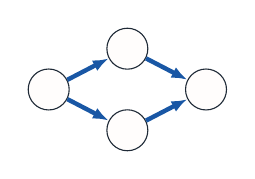
\begin{tikzpicture}[scale=0.74, every node/.style={circle,draw=Ink,fill=PaperCard,minimum size=0.52cm,inner sep=0pt}]
    \node (a) at (0,0) {};
    \node (b) at (1.35,0.7) {};
    \node (c) at (1.35,-0.7) {};
    \node (d) at (2.7,0) {};
    \draw[CausalBlue,line width=1.6pt,-{Latex[length=2mm]}] (a) -- (b);
    \draw[CausalBlue,line width=1.6pt,-{Latex[length=2mm]}] (a) -- (c);
    \draw[CausalBlue,line width=1.6pt,-{Latex[length=2mm]}] (b) -- (d);
    \draw[CausalBlue,line width=1.6pt,-{Latex[length=2mm]}] (c) -- (d);
  \end{tikzpicture}
}

\newcommand{\MiniGraphNovelty}{%
  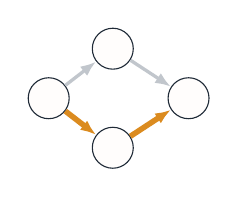
\begin{tikzpicture}[scale=0.74, every node/.style={circle,draw=Ink,fill=PaperCard,minimum size=0.52cm,inner sep=0pt}]
    \node (a) at (0,0) {};
    \node (b) at (1.1,0.85) {};
    \node (c) at (1.1,-0.85) {};
    \node (d) at (2.4,0) {};
    \draw[Muted!45,line width=1.2pt,-{Latex[length=2mm]}] (a) -- (b);
    \draw[Muted!45,line width=1.2pt,-{Latex[length=2mm]}] (b) -- (d);
    \draw[NonCausalOrange,line width=2pt,-{Latex[length=2mm]}] (a) -- (c);
    \draw[NonCausalOrange,line width=2pt,-{Latex[length=2mm]}] (c) -- (d);
  \end{tikzpicture}
}

\newcommand{\MiniGraphPosition}{%
  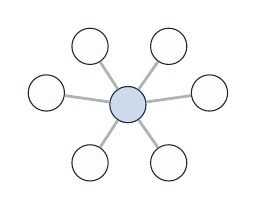
\begin{tikzpicture}[scale=0.74, every node/.style={circle,draw=Ink,fill=PaperCard,minimum size=0.46cm,inner sep=0pt}]
    \node[fill=CausalBlue!22] (center) at (1.4,0) {};
    \node (a) at (0,0.2) {};
    \node (b) at (0.75,1.0) {};
    \node (c) at (2.1,1.0) {};
    \node (d) at (2.8,0.2) {};
    \node (e) at (2.1,-1.0) {};
    \node (f) at (0.75,-1.0) {};
    \foreach \x in {a,b,c,d,e,f}{
      \draw[Muted!60,line width=1pt] (center) -- (\x);
    }
  \end{tikzpicture}
}

\setbeamertemplate{footline}{%
  \leavevmode%
  \hbox{%
    \begin{beamercolorbox}[wd=.8\paperwidth,ht=2.8ex,dp=1.3ex,leftskip=0.8cm]{footline}%
      \textbf{Causal Claims in Economics} \hspace{0.5em}\textcolor{Muted}{|} \hspace{0.5em}\insertsectionhead
    \end{beamercolorbox}%
    \begin{beamercolorbox}[wd=.2\paperwidth,ht=2.8ex,dp=1.3ex,rightskip=0.8cm plus1fil]{footline}%
      \insertframenumber/\inserttotalframenumber
    \end{beamercolorbox}%
  }%
}

\title{Causal Claims in Economics}
\subtitle{From prose to claim graphs for 44,852 working papers}
\author{Prashant Garg \and Thiemo Fetzer}
\date{\today}

\begin{document}

\section{Why This Problem Exists}

\begin{frame}[plain]
  \begin{tikzpicture}[remember picture,overlay]
    \fill[PaperSand] (current page.south west) rectangle ([xshift=5.15cm]current page.north west);
    \fill[CausalBlue!8] ([xshift=7.9cm]current page.south west) rectangle (current page.north east);
    \fill[AccentCoral!14] ([xshift=12.2cm,yshift=0.9cm]current page.south west) circle (1.85cm);
    \fill[AccentTeal!12] ([xshift=13.5cm,yshift=5.8cm]current page.south west) circle (1.2cm);
  \end{tikzpicture}

  \begin{columns}[T,onlytextwidth]
    \begin{column}{0.58\textwidth}
      \vspace{1.6cm}
      {\fontsize{28}{33}\selectfont\bfseries Causal Claims in Economics\par}

      \vspace{0.48cm}
      \begin{tabular}{@{}p{0.42\linewidth}p{0.42\linewidth}@{}}
        {\small\bfseries Prashant Garg} & {\small\bfseries Thiemo Fetzer} \\
        {\small\textcolor{Muted}{Imperial College London}} & {\small\textcolor{Muted}{Warwick / Bonn / CEPR}}
      \end{tabular}

      \vfill
      {\small\textcolor{Muted}{Project: }\href{https://www.causal.claims}{\textcolor{CausalBlue}{\textbf{causal.claims}}}}
    \end{column}
    \begin{column}{0.38\textwidth}
      \vspace{0.72cm}
      \begin{tikzpicture}
        \node[
          fill=white,
          draw=LineSoft,
          line width=0.8pt,
          rounded corners=12pt,
          inner sep=6pt
        ] {\begin{minipage}{0.92\linewidth}\centering
            \resizebox{\linewidth}{!}{\begin{tikzpicture}
  \node[cg node, text width=2.20cm, minimum height=7mm, inner sep=1.5pt] (micro) at (-3.0,0.2) {Microfinance access\\(G21)};
  \node[cg node, text width=2.20cm, minimum height=7mm, inner sep=1.5pt] (social) at (-0.4,1.9) {Social outcomes\\(I24)};
  \node[cg node, text width=2.20cm, minimum height=7mm, inner sep=1.5pt] (borrow) at (1.2,1.3) {Borrowing rates\\(E43)};
  \node[cg node, text width=2.20cm, minimum height=7mm, inner sep=1.5pt] (newbiz) at (1.4,0.2) {Business creation\\(L26)};
  \node[cg node, text width=2.20cm, minimum height=7mm, inner sep=1.5pt] (cons) at (1.0,-1.0) {Consumption\\patterns (D10)};
  \node[cg node, text width=2.20cm, minimum height=7mm, inner sep=1.5pt] (invest) at (-3.0,-1.85) {Investment in\\existing firms (G31)};
  \node[cg node, text width=2.20cm, minimum height=7mm, inner sep=1.5pt] (profits) at (-0.15,-1.85) {Average profits\\(D33)};

  \draw[cg causal] (micro) -- (social);
  \draw[cg causal] (micro) -- (borrow);
  \draw[cg causal] (micro) -- (newbiz);
  \draw[cg causal] (micro) -- (cons);
  \draw[cg causal] (micro) -- (invest);
  \draw[cg causal] (invest) -- (profits);
\end{tikzpicture}
}
          \end{minipage}};
      \end{tikzpicture}

      \vspace{0.16cm}
      \chip[CausalBlue]{Example claim graph}
      \hspace{0.12cm}
      \ghost{Banerjee et al. (2015)}
    \end{column}
  \end{columns}
\end{frame}

\begin{frame}[t]{Economics has a representation problem}
  \begin{columns}[T,onlytextwidth]
    \begin{column}{0.43\textwidth}
      \vspace{0.06cm}
      {\fontsize{18}{21}\selectfont\bfseries The bottleneck has moved.\par}
      \vspace{0.16cm}
      {\normalsize It is now cheaper to produce papers than to organize what they actually claim.\par}

      \vspace{0.24cm}
      \begin{overlayarea}{\linewidth}{0.39\textheight}
        \only<2->{\Card{0.88\linewidth}{Too much prose}{Working-paper ecosystems scale easily; claims do not.}}

        \vspace{0.12cm}
        \only<4->{\Card{0.88\linewidth}{Too little structure}{Claims, mechanisms, and evidence types sit inside narrative text instead of comparable objects.}}
      \end{overlayarea}
    \end{column}
    \begin{column}{0.54\textwidth}
      \vspace{0.14cm}
      \begin{overlayarea}{\linewidth}{0.66\textheight}
        \only<3->{\CompactCard{0.92\linewidth}{1. Reading does not scale}{You can skim thousands of titles. You cannot manually normalize thousands of claim structures.}}

        \vspace{0.15cm}
        \only<5->{\CompactCard{0.92\linewidth}{2. Search is shallow}{Topic tags tell us what a paper is about; they do not store which relationship is claimed, by which design, and through which mechanism.}}

        \vspace{0.15cm}
        \only<6->{\CompactCard{0.92\linewidth}{3. Synthesis stays manual}{If cumulative science matters, prose alone is a poor storage format for comparison and reuse.}}
      \end{overlayarea}
    \end{column}
  \end{columns}
\end{frame}

\begin{frame}[t]{Why prose is the wrong storage layer}
  \begin{columns}[T,onlytextwidth]
    \begin{column}{0.49\textwidth}
      \begin{overlayarea}{\linewidth}{0.46\textheight}
        \visible<1->{\CompactCard{0.96\linewidth}{What the literature gives us}{
          \textbf{Question:} often implicit, spread across abstract and introduction.\par\medskip
          \textbf{Mechanism:} buried in chains of sentences and section-specific language.\par\medskip
          \textbf{Evidence:} mixed together with rhetoric, tables, and design discussion.}}
      \end{overlayarea}

      \vspace{0.08cm}
      \begin{overlayarea}{\linewidth}{0.18\textheight}
        \visible<3->{\CompactCard[PaperSand]{0.96\linewidth}{The result}{
          Great papers are easy to cite but hard to \textit{parse} into a comparable, machine-readable object.}}
      \end{overlayarea}
    \end{column}
    \begin{column}{0.47\textwidth}
      \begin{overlayarea}{\linewidth}{0.46\textheight}
        \visible<2->{\CompactCard{0.95\linewidth}{What cumulative science needs}{
          \textbf{Nodes:} standardized economic concepts.\par\medskip
          \textbf{Edges:} explicit source to sink relationships.\par\medskip
          \textbf{Evidence labels:} causal design, non-causal support, tentativeness, novelty, and position.}}
      \end{overlayarea}

      \vspace{0.08cm}
      \begin{overlayarea}{\linewidth}{0.22\textheight}
        \visible<4->{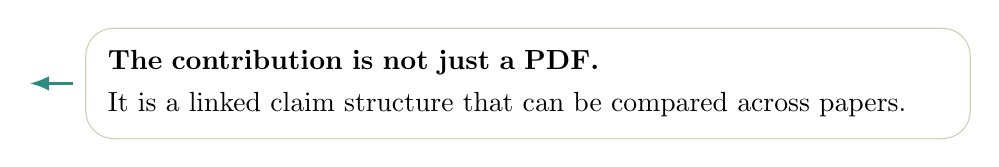
\begin{tikzpicture}[>=Latex]
          \node[
            fill=white,
            draw=LineSoft,
            rounded corners=10pt,
            inner sep=8pt,
            text width=0.88\linewidth,
            align=left
          ] (box) {\textbf{The contribution is not just a PDF.}\par\smallskip It is a linked claim structure that can be compared across papers.};
          \draw[AccentTeal,line width=1.2pt,-{Latex[length=2.5mm]}] ([xshift=-0.16cm]box.west) -- ++(-0.55cm,0);
        \end{tikzpicture}}
      \end{overlayarea}
    \end{column}
  \end{columns}
\end{frame}

\section{What A Claim Graph Is}

\SectionDivider{Claim graphs}{A paper as a graph}{What the object looks like before the pipeline.}

\begin{frame}[t]{A claim graph is a paper-level object}
  \begin{columns}[T,onlytextwidth]
    \begin{column}{0.5\textwidth}
      \vspace{0.12cm}
      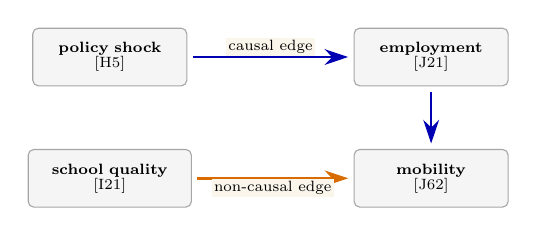
\begin{tikzpicture}[>=Latex, scale=0.77, transform shape]
        \node[cg node,text width=2.4cm,minimum height=0.95cm] (a) at (0.0,1.0) {\textbf{policy shock}\\[-1pt] [H5]};
        \node[cg node,text width=2.4cm,minimum height=0.95cm] (b) at (5.3,1.0) {\textbf{employment}\\[-1pt] [J21]};
        \node[cg node,text width=2.4cm,minimum height=0.95cm] (c) at (5.3,-1.0) {\textbf{mobility}\\[-1pt] [J62]};
        \node[cg node,text width=2.55cm,minimum height=0.95cm] (d) at (0.0,-1.0) {\textbf{school quality}\\[-1pt] [I21]};

        \draw[cg causal] (a.east) -- node[above,fill=PaperBg,inner sep=1pt]{\scriptsize causal edge} (b.west);
        \draw[cg causal] (b.south) -- (c.north);
        \draw[cg noncausal] (d.east) -- node[below,fill=PaperBg,inner sep=1pt]{\scriptsize non-causal edge} (c.west);
      \end{tikzpicture}
    \end{column}
    \begin{column}{0.45\textwidth}
      \vspace{0.02cm}
      \begin{overlayarea}{\linewidth}{0.18\textheight}
        \only<1->{\CompactCard{0.98\linewidth}{Nodes}{
          Economic concepts mapped to a common ontology: here, JEL codes.}}
      \end{overlayarea}

      \vspace{0.03cm}
      \begin{overlayarea}{\linewidth}{0.18\textheight}
        \only<2->{\CompactCard{0.98\linewidth}{Edges}{
          Directed source-to-sink relationships as stated by the paper.}}
      \end{overlayarea}

      \vspace{0.03cm}
      \begin{overlayarea}{\linewidth}{0.22\textheight}
        \only<3->{\CompactCard{0.98\linewidth}{Evidence annotation}{
          Each edge stores whether support comes from DiD, IV, RCT, RDD, synthetic control, or non-causal evidence.}}
      \end{overlayarea}
    \end{column}
  \end{columns}

  \figurecaptionbar{This is the core move: represent argumentative structure in a comparable, aggregable form.}
\end{frame}

\begin{frame}[t,label=main-graphs]{Before the pipeline, make it concrete}
  \begin{columns}[T,onlytextwidth]
    \begin{column}{0.48\textwidth}
      \begin{tikzpicture}
        \node[
          fill=white,
          draw=LineSoft,
          line width=0.7pt,
          rounded corners=10pt,
          inner sep=6pt
        ] {\begin{minipage}{0.93\linewidth}\centering
            \resizebox{\linewidth}{!}{\begin{tikzpicture}
  \node[cg node, text width=2.20cm, minimum height=7mm, inner sep=1.5pt] (par) at (-3.0,1.55) {Parent income\\(D31)};
  \node[cg node, text width=2.20cm, minimum height=7mm, inner sep=1.5pt] (ineq) at (-2.8,0.3) {Income inequality\\(D31)};
  \node[cg node, text width=2.20cm, minimum height=7mm, inner sep=1.5pt] (school) at (-2.7,-0.8) {School quality\\(I21)};
  \node[cg node, text width=2.20cm, minimum height=7mm, inner sep=1.5pt] (fam) at (-2.4,-1.9) {Family stability\\(J12)};
  \node[cg node, text width=2.20cm, minimum height=7mm, inner sep=1.5pt] (seg) at (0.0,-2.1) {Residential\\segregation (R23)};
  \node[cg node, text width=2.20cm, minimum height=7mm, inner sep=1.5pt] (soc) at (2.4,-1.6) {Social capital\\(Z13)};
  \node[cg node, text width=2.20cm, minimum height=7mm, inner sep=1.5pt] (mob) at (0.3,-0.05) {Upward mobility\\(J62)};
  \node[cg node, text width=2.20cm, minimum height=7mm, inner sep=1.5pt] (child) at (3.0,1.55) {Child income\\(J13)};

  \draw[cg noncausal] (par) -- (child);
  \draw[cg noncausal] (ineq) -- (mob);
  \draw[cg noncausal] (school) -- (mob);
  \draw[cg noncausal] (fam) -- (mob);
  \draw[cg noncausal] (seg) -- (mob);
  \draw[cg noncausal] (soc) -- (mob);
  \draw[cg noncausal] (mob) to[out=30,in=120,looseness=8] (mob);
\end{tikzpicture}
}
          \end{minipage}};
      \end{tikzpicture}
      \vspace{0.12cm}
      \chip[NonCausalOrange]{Chetty et al. (2014)}
      \hspace{0.15cm}
      \ghost{Broad correlational map around upward mobility}
    \end{column}
    \begin{column}{0.48\textwidth}
      \begin{tikzpicture}
        \node[
          fill=white,
          draw=LineSoft,
          line width=0.7pt,
          rounded corners=10pt,
          inner sep=6pt
        ] {\begin{minipage}{0.93\linewidth}\centering
            \resizebox{\linewidth}{!}{\begin{tikzpicture}
  \node[cg node, text width=2.20cm, minimum height=7mm, inner sep=1.5pt] (micro) at (-3.0,0.2) {Microfinance access\\(G21)};
  \node[cg node, text width=2.20cm, minimum height=7mm, inner sep=1.5pt] (social) at (-0.4,1.9) {Social outcomes\\(I24)};
  \node[cg node, text width=2.20cm, minimum height=7mm, inner sep=1.5pt] (borrow) at (1.2,1.3) {Borrowing rates\\(E43)};
  \node[cg node, text width=2.20cm, minimum height=7mm, inner sep=1.5pt] (newbiz) at (1.4,0.2) {Business creation\\(L26)};
  \node[cg node, text width=2.20cm, minimum height=7mm, inner sep=1.5pt] (cons) at (1.0,-1.0) {Consumption\\patterns (D10)};
  \node[cg node, text width=2.20cm, minimum height=7mm, inner sep=1.5pt] (invest) at (-3.0,-1.85) {Investment in\\existing firms (G31)};
  \node[cg node, text width=2.20cm, minimum height=7mm, inner sep=1.5pt] (profits) at (-0.15,-1.85) {Average profits\\(D33)};

  \draw[cg causal] (micro) -- (social);
  \draw[cg causal] (micro) -- (borrow);
  \draw[cg causal] (micro) -- (newbiz);
  \draw[cg causal] (micro) -- (cons);
  \draw[cg causal] (micro) -- (invest);
  \draw[cg causal] (invest) -- (profits);
\end{tikzpicture}
}
          \end{minipage}};
      \end{tikzpicture}
      \vspace{0.12cm}
      \chip[CausalBlue]{Banerjee et al. (2015)}
      \hspace{0.15cm}
      \ghost{Compact causal chain with RCT-backed outcomes}
    \end{column}
  \end{columns}

  \vspace{0.05cm}
  \figurecaptionbar{Same discipline, same status, very different claim architecture.}
\end{frame}

\begin{frame}[t]{Two more landmark graphs}
  \begin{columns}[T,onlytextwidth]
    \begin{column}{0.48\textwidth}
      \begin{tikzpicture}
        \node[
          fill=white,
          draw=LineSoft,
          rounded corners=10pt,
          inner sep=6pt
        ] {\begin{minipage}{0.93\linewidth}\centering
            \resizebox{\linewidth}{!}{\begin{tikzpicture}
  \node[cg node, text width=2.30cm, minimum height=7.5mm, inner sep=1.6pt] (shock) at (-2.9,0.0) {Idiosyncratic shocks\\(D89)};
  \node[cg node, text width=2.30cm, minimum height=7.5mm, inner sep=1.6pt] (prop) at (0.7,1.1) {Propagation through\\the economy (E10)};
  \node[cg node, text width=2.30cm, minimum height=7.5mm, inner sep=1.6pt] (macro) at (0.7,-1.1) {Macroeconomic\\dynamics (E19)};

  \draw[cg noncausal] (shock) -- (prop);
  \draw[cg noncausal] (shock) -- (macro);
\end{tikzpicture}
}
          \end{minipage}};
      \end{tikzpicture}
      \vspace{0.1cm}
      \chip[NonCausalOrange]{Gabaix (2011)}
      \hspace{0.12cm}
      \ghost{Compact non-causal mechanism structure}
    \end{column}
    \begin{column}{0.48\textwidth}
      \begin{tikzpicture}
        \node[
          fill=white,
          draw=LineSoft,
          rounded corners=10pt,
          inner sep=6pt
        ] {\begin{minipage}{0.93\linewidth}\centering
            \resizebox{\linewidth}{!}{\begin{tikzpicture}
  \node[cg node, text width=2.30cm, minimum height=7.5mm, inner sep=1.6pt] (tariff) at (-2.8,1.0) {Lower input\\tariffs (F14)};
  \node[cg node, text width=2.30cm, minimum height=7.5mm, inner sep=1.6pt] (imports) at (-2.8,-1.0) {New imported\\intermediates (Y20)};
  \node[cg node, text width=2.30cm, minimum height=7.5mm, inner sep=1.6pt] (prod) at (0.8,1.5) {Higher firm\\productivity (D21)};
  \node[cg node, text width=2.30cm, minimum height=7.5mm, inner sep=1.6pt] (scope) at (0.8,0.2) {Expanded product\\scope (L25)};
  \node[cg node, text width=2.30cm, minimum height=7.5mm, inner sep=1.6pt] (domestic) at (0.8,-1.2) {New domestic\\products (L68)};

  \draw[cg causal] (tariff) -- (prod);
  \draw[cg causal] (tariff) -- (scope);
  \draw[cg noncausal] (imports) -- (domestic);
\end{tikzpicture}
}
          \end{minipage}};
      \end{tikzpicture}
      \vspace{0.1cm}
      \chip[CausalBlue]{Goldberg et al. (2010)}
      \hspace{0.12cm}
      \ghost{Mixed causal and non-causal claim structure}
    \end{column}
  \end{columns}

  \vspace{0.04cm}
  \figurecaptionbar{The object captures different architectures, not just different topics.}
\end{frame}

\begin{frame}[t]{What the object captures -- and what it does not}
  \begin{columns}[T,onlytextwidth]
    \begin{column}{0.48\textwidth}
      \only<1->{\Card{0.97\linewidth}{What claim graphs capture}{
        \ding{51}\ Which concepts a paper connects\par
        \ding{51}\ Whether support is causal or non-causal\par
        \ding{51}\ Complexity, novelty, and topic position\par
        \ding{51}\ Paper-level structure that can be compared at scale}}
    \end{column}
    \begin{column}{0.48\textwidth}
      \only<2->{\Card[PaperSand]{0.97\linewidth}{What claim graphs do not do}{
        \ding{55}\ They do not decide whether a claim is true\par
        \ding{55}\ They do not recover every nuance of variable wording\par
        \ding{55}\ They do not eliminate the need for validation and judgment}}
    \end{column}
  \end{columns}

  \vspace{0.16cm}
  \only<3->{\Card{0.99\linewidth}{Interpretation rule}{
    This is measurement infrastructure. It extracts what papers \emph{state} and how they support it. That is already a large step forward.}}
\end{frame}

\section{How We Built It}

\SectionDivider{Measurement}{Build the infrastructure}{How the retrieval pipeline turns papers into claim graphs.}

\begin{frame}[t]{Corpus, scope, and design choices}
  \begin{columns}[T,onlytextwidth]
    \begin{column}{0.23\textwidth}
      \only<1->{\StatCard{0.96\linewidth}{44,852}{NBER + CEPR working papers}}
    \end{column}
    \begin{column}{0.23\textwidth}
      \only<2->{\StatCard{0.96\linewidth}{1980--2023}{Four decades of economics}}
    \end{column}
    \begin{column}{0.23\textwidth}
      \only<3->{\StatCard{0.96\linewidth}{30 pages}{Fixed input window per paper}}
    \end{column}
    \begin{column}{0.23\textwidth}
      \only<4->{\StatCard{0.96\linewidth}{Sep 2024}{Publication + citation snapshot}}
    \end{column}
  \end{columns}

  \vspace{0.3cm}
  \begin{columns}[T,onlytextwidth]
    \begin{column}{0.54\textwidth}
      \only<5->{\Card{0.98\linewidth}{Why the first 30 pages?}{
        In economics, the abstract, introduction, identification strategy, and main results usually contain the paper's central claims. A fixed cap keeps decades comparable as papers lengthen.}
      }
    \end{column}
    \begin{column}{0.38\textwidth}
      \only<6->{\Card[PaperSand]{0.98\linewidth}{What is intentionally narrow}{
        Causal edges are defined conservatively: DiD, IV, RCT, RDD, event-study-style DiD/TWFE implementations, and synthetic control.}
      }
    \end{column}
  \end{columns}
\end{frame}

\begin{frame}[t]{Extraction pipeline: retrieve, standardize, aggregate}
  \begin{center}
    \begin{tikzpicture}
      \node[
        fill=white,
        draw=LineSoft,
        line width=0.7pt,
        rounded corners=10pt,
        inner sep=6pt
      ] {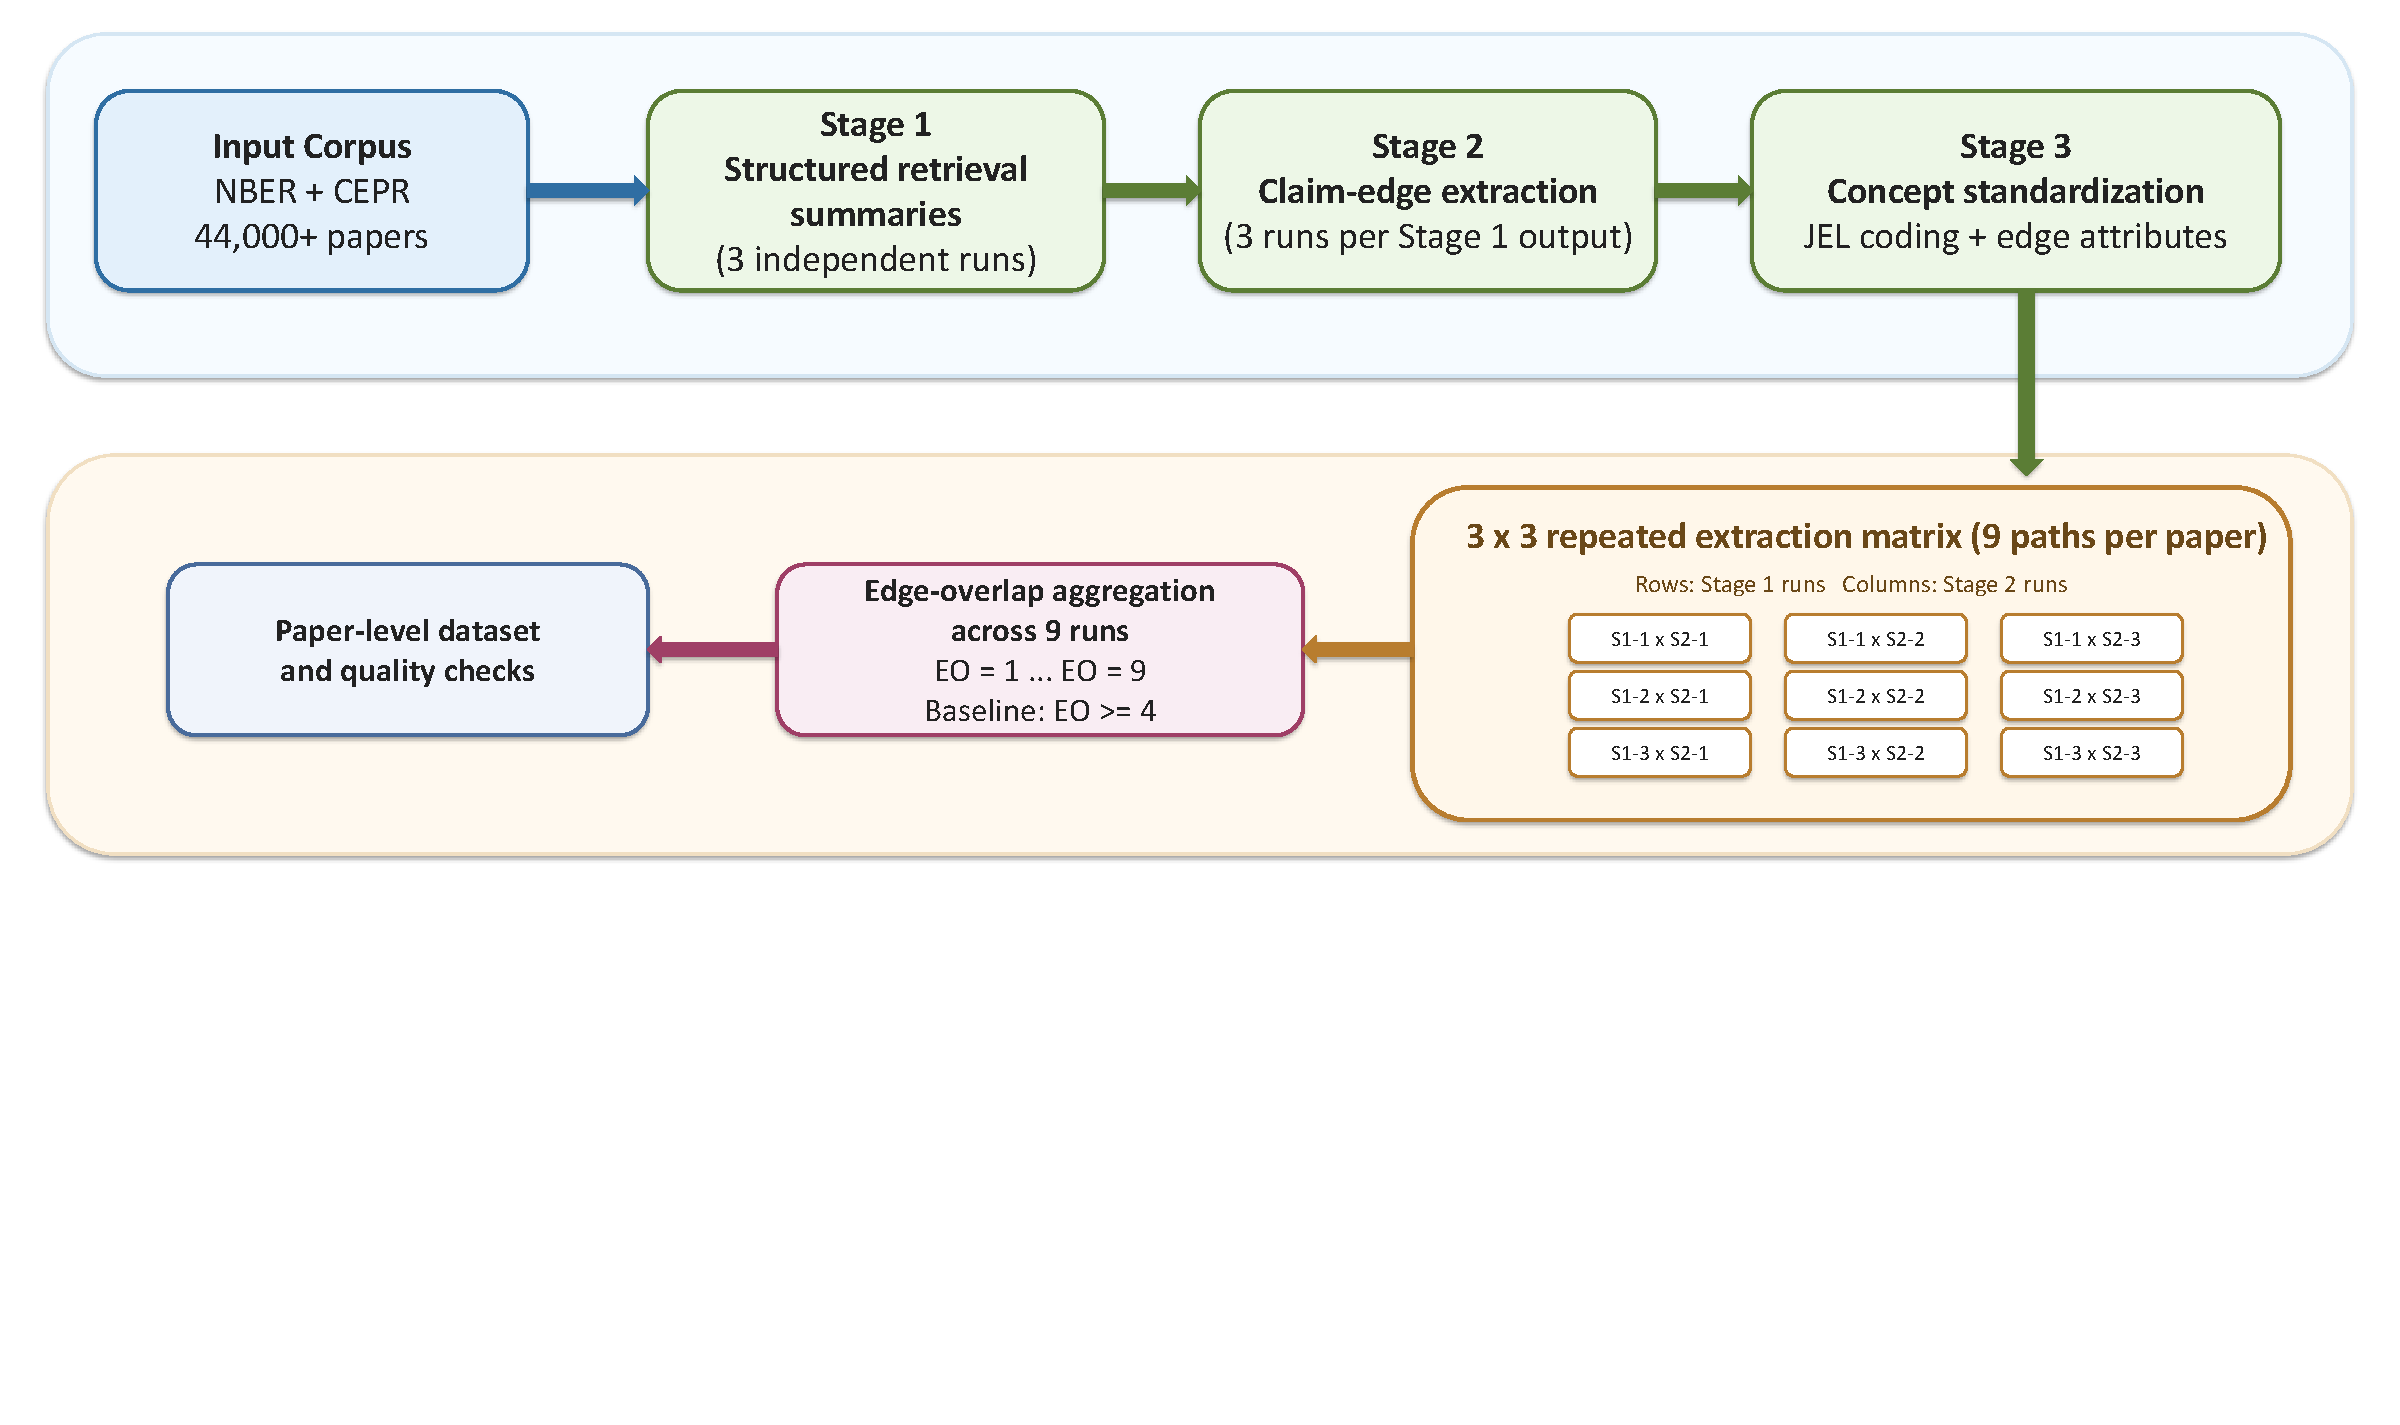
\includegraphics[width=0.79\linewidth,trim=0 8cm 0 0,clip]{pipeline_flowchart_master_editable.pdf}};
    \end{tikzpicture}
  \end{center}

  \vspace{0.12cm}
  \begin{overlayarea}{\linewidth}{0.14\textheight}
    \only<1>{\StageCard{Stage 1: qualitative curation}{Three first-30-page summaries recover the question, design cues, and claim snippets.}}
    \only<2>{\StageCard{Stage 2: graph extraction}{Convert each summary into labeled source-to-sink edges.}}
    \only<3>{\StageCard{Stage 3: concept standardization}{Map endpoints to JEL concepts.}}
    \only<4->{\StageCard{Stage 4: EO aggregation}{Retain recurring edges; EO >= 4 is the baseline.}}
  \end{overlayarea}
\end{frame}

\begin{frame}[t]{Edge-overlap makes precision and recall explicit}
  \begin{columns}[T,onlytextwidth]
    \begin{column}{0.42\textwidth}
      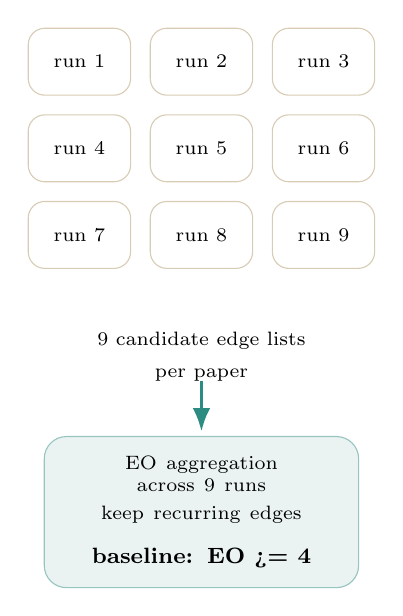
\begin{tikzpicture}[>=Latex]
        \foreach \r in {0,1,2} {
          \foreach \c in {0,1,2} {
            \node[
              draw=LineSoft,
              fill=white,
              rounded corners=6pt,
              minimum width=1.3cm,
              minimum height=0.85cm
            ] (n\r\c) at (\c*1.55,-\r*1.1) {\scriptsize run \the\numexpr\r*3+\c+1\relax};
          }
        }
        \node[align=center] at (1.55,-3.75) {\scriptsize 9 candidate edge lists\\[-0.05em]\scriptsize per paper};
        \draw[AccentTeal,line width=1.4pt,-{Latex[length=3mm]}] (1.55,-4.05) -- (1.55,-4.7);
        \node[
          draw=AccentTeal!50,
          fill=AccentTeal!10,
          rounded corners=8pt,
          text width=3.5cm,
          inner sep=7pt,
          align=center
        ] (agg) at (1.55,-5.72) {\scriptsize EO aggregation across 9 runs\\[0.08cm]\scriptsize keep recurring edges\\[0.14cm]\footnotesize\bfseries baseline: EO >= 4};
      \end{tikzpicture}
    \end{column}
    \begin{column}{0.54\textwidth}
      \Card{0.98\linewidth}{Why this matters}{
        A single LLM pass is a noisy measurement. Repeating the same constrained extraction and retaining overlapping edges makes the trade-off transparent rather than mystical.}

      \vspace{0.22cm}
      \Card[PaperSand]{0.98\linewidth}{Interpretation}{
        Lower EO keeps more candidate edges but accepts more noise. Higher EO suppresses fragile edges but thins the graph. The paper uses EO >= 4 as the operating point.}
    \end{column}
  \end{columns}
\end{frame}

\begin{frame}[t,label=main-validation]{Why trust the measurement at all?}
  \begin{columns}[T,onlytextwidth]
    \begin{column}{0.32\textwidth}
      \Card{0.96\linewidth}{External benchmark 1}{
        Match method and field labels against the Brodeur et al.\ dataset of leading economics papers.}
    \end{column}
    \begin{column}{0.32\textwidth}
      \Card{0.96\linewidth}{External benchmark 2}{
        Compare causes, effects, and exogenous variation with the Plausibly Exogenous Galore dataset.}
    \end{column}
    \begin{column}{0.32\textwidth}
      \Card{0.96\linewidth}{Internal audit}{
        Re-extract edges from verbatim snippets only and inspect the precision--recall trade-off across EO thresholds.}
    \end{column}
  \end{columns}

  \vspace{0.32cm}
  \Card[PaperSand]{0.99\linewidth}{Bottom line}{
    Treat this as a measurement system, not an oracle. The paper validates the retrieval on method labels, concept alignment, exogenous variation, and stability under stricter overlap thresholds.}

  \vspace{0.15cm}
  {\scriptsize\bfseries More details:\hspace{0.2cm}}
  \JumpButton{app-brodeur}{Brodeur}
  \hspace{0.12cm}
  \JumpButton{app-plausibly}{Plausibly Exogenous}
  \hspace{0.12cm}
  \JumpButton{app-snippet}{Snippet / EO audit}
\end{frame}

\BridgeSlide{}{What does the measurement show?}{Start with how causal evidence changed across economics.}

\section{What Changed In Economics}

\SectionDivider{Descriptive results}{What changed in economics?}{The claim-level view of the credibility revolution.}

\begin{frame}[t,label=main-trend]{The share of causal edges rises sharply}
  \begin{columns}[T,onlytextwidth]
    \begin{column}{0.68\textwidth}
      \begin{tikzpicture}
        \node[
          fill=white,
          draw=LineSoft,
          rounded corners=10pt,
          inner sep=6pt
        ] {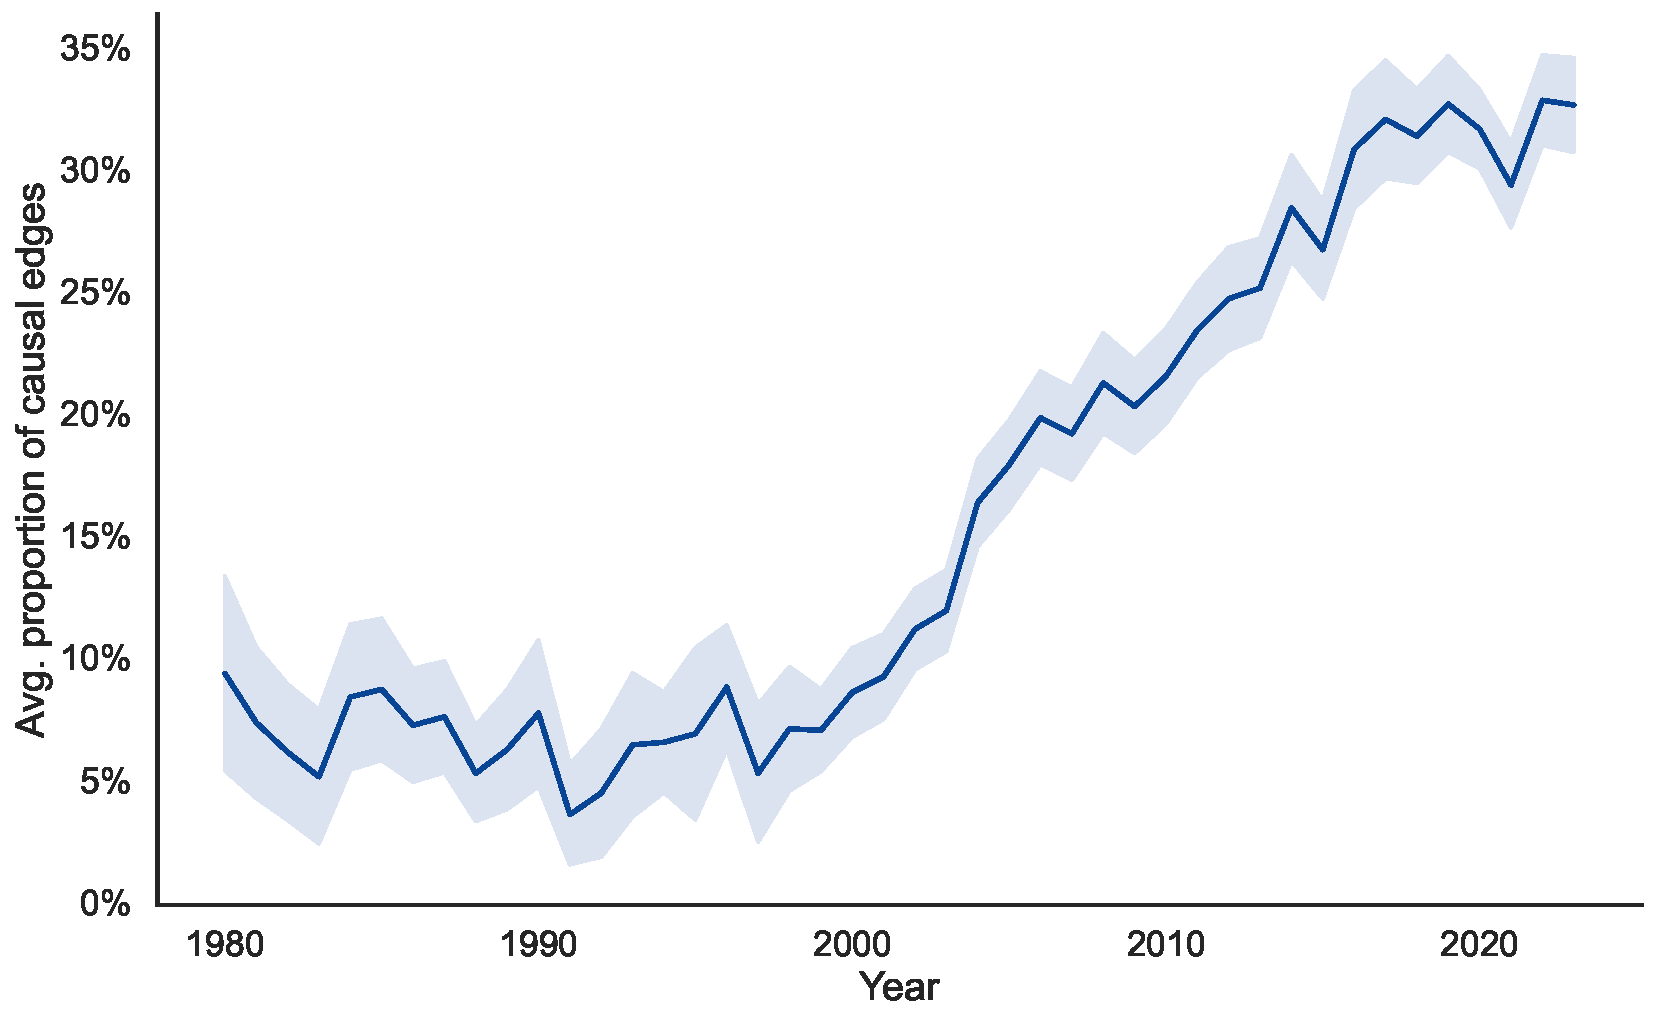
\includegraphics[width=0.98\linewidth]{prop_causal_edges_over_time.pdf}};
      \end{tikzpicture}
    \end{column}
    \begin{column}{0.3\textwidth}
      \vspace{0.08cm}
      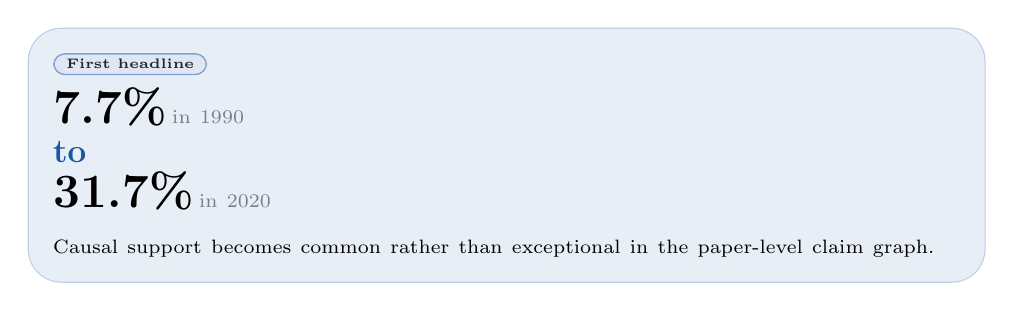
\begin{tikzpicture}
        \node[
          fill=CausalBlue!10,
          draw=CausalBlue!28,
          rounded corners=12pt,
          inner sep=9pt,
          text width=0.95\linewidth,
          align=left
        ] {\chip[CausalBlue]{First headline}\par
          \vspace{0.12cm}
          {\fontsize{19}{21}\selectfont\bfseries 7.7\%}\hspace{0.2em}{\scriptsize\textcolor{Muted}{in 1990}}\par
          \vspace{0.08cm}
          {\large\textcolor{CausalBlue}{\bfseries to}}\par
          \vspace{0.08cm}
          {\fontsize{19}{21}\selectfont\bfseries 31.7\%}\hspace{0.2em}{\scriptsize\textcolor{Muted}{in 2020}}\par
          \vspace{0.16cm}
          \scriptsize Causal support becomes common rather than exceptional in the paper-level claim graph.};
      \end{tikzpicture}
    \end{column}
  \end{columns}

  \figurecaptionbar{Why this matters: the credibility revolution is visible not just in methods used by papers, but in the share of relationships backed by causal designs.}

  \vspace{0.03cm}
  \hfill\JumpButton{app-eo-trend}{EO robustness}
\end{frame}

\begin{frame}[t]{The rise is broad -- but not uniform across fields}
  \begin{center}
    \begin{tikzpicture}
      \node[
        fill=white,
        draw=LineSoft,
        rounded corners=10pt,
        inner sep=6pt
      ] {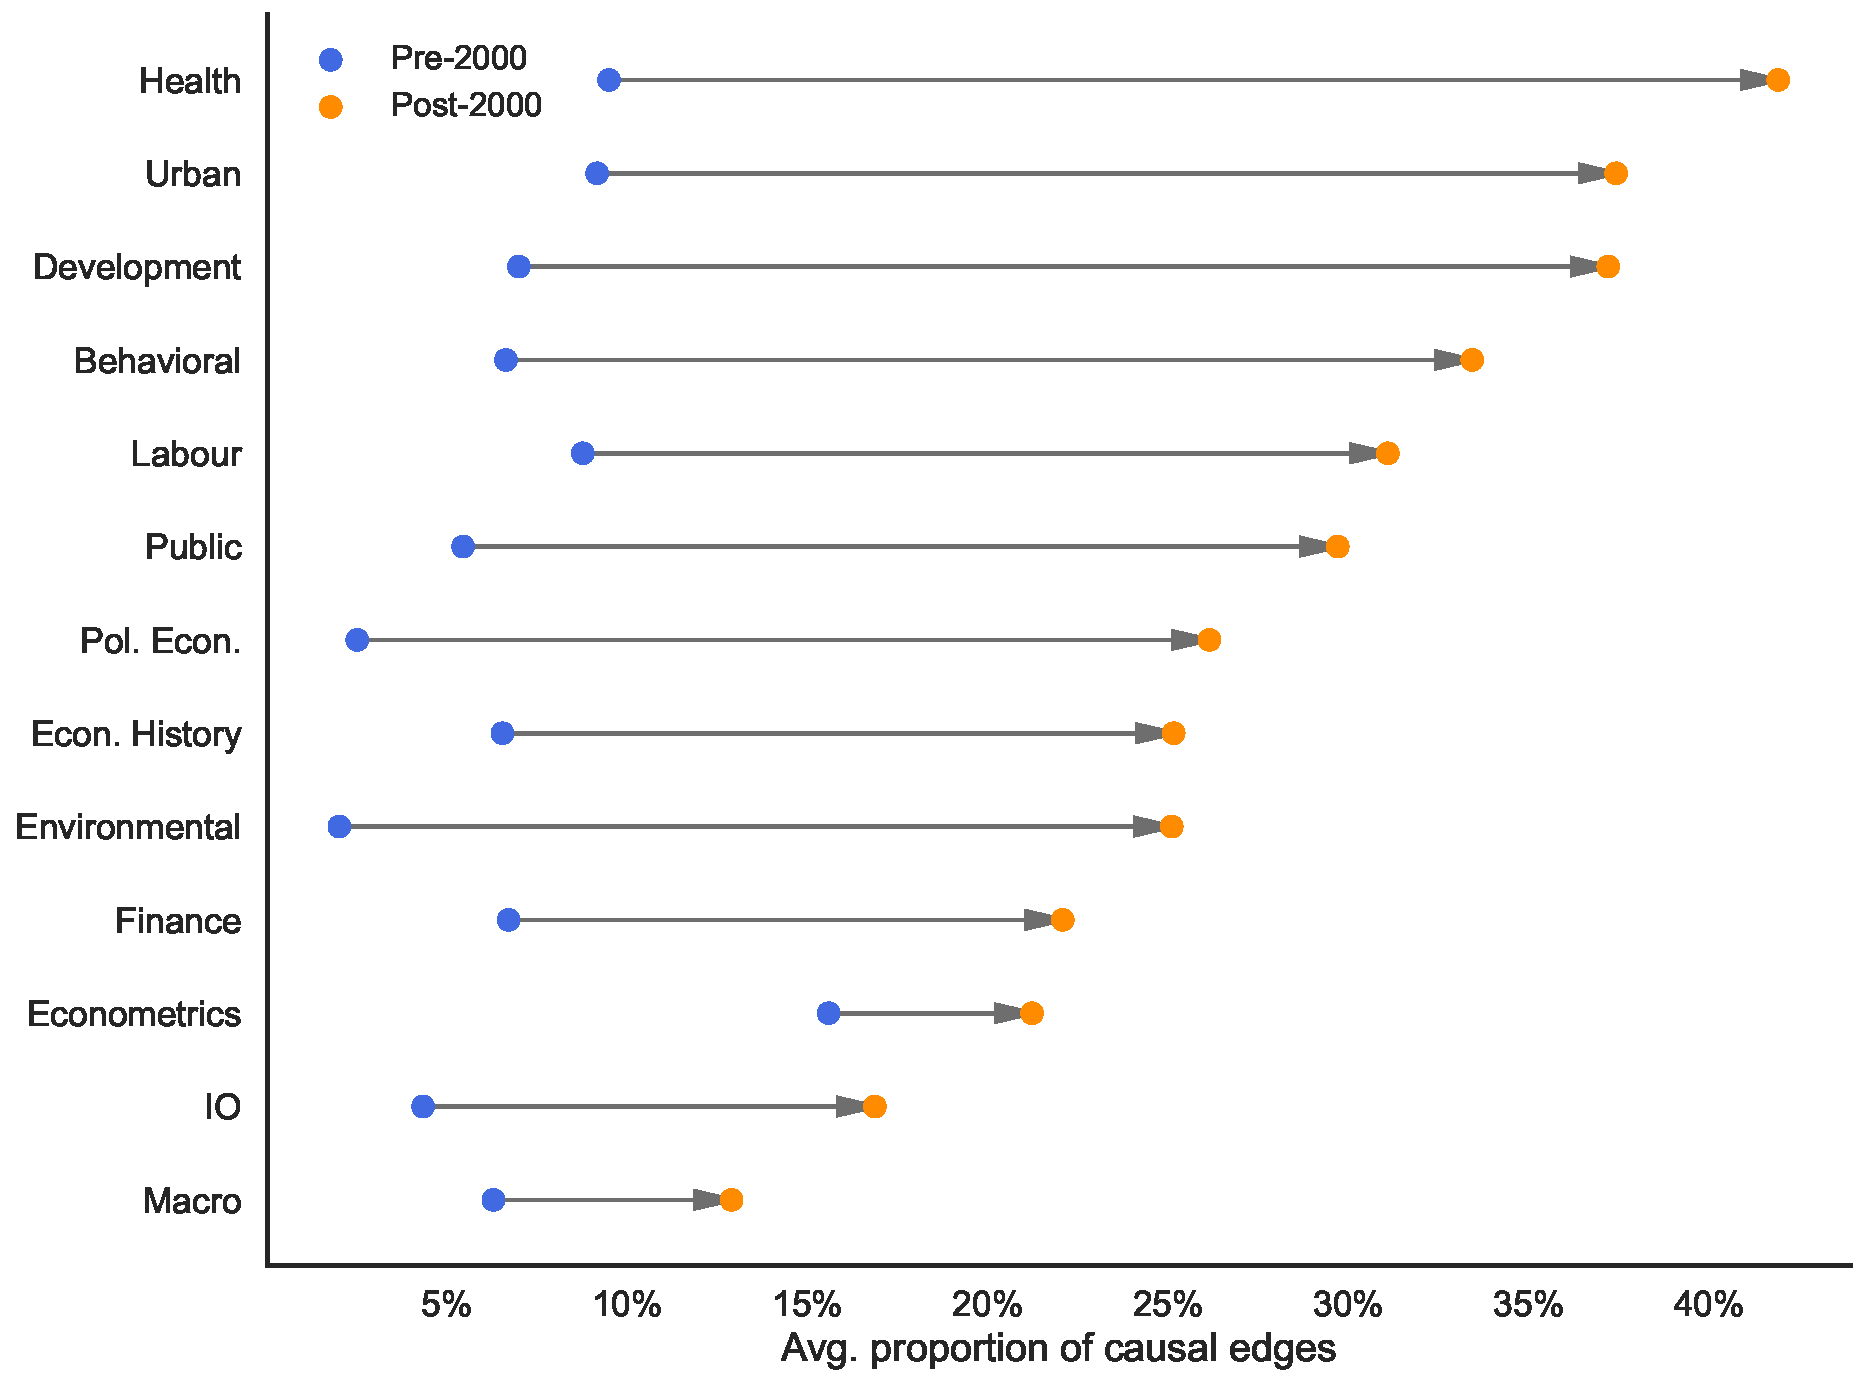
\includegraphics[width=0.85\linewidth,height=0.68\textheight,keepaspectratio]{prop_causal_edges_by_field_period.pdf}};
    \end{tikzpicture}
  \end{center}

  \figurecaptionbar{The diffusion is discipline-wide, but still shaped by field-specific data environments and identification traditions.}
\end{frame}

\begin{frame}[t]{Method diffusion confirms the same story}
  \begin{center}
    \begin{tikzpicture}
      \node[
        fill=white,
        draw=LineSoft,
        rounded corners=10pt,
        inner sep=6pt
      ] {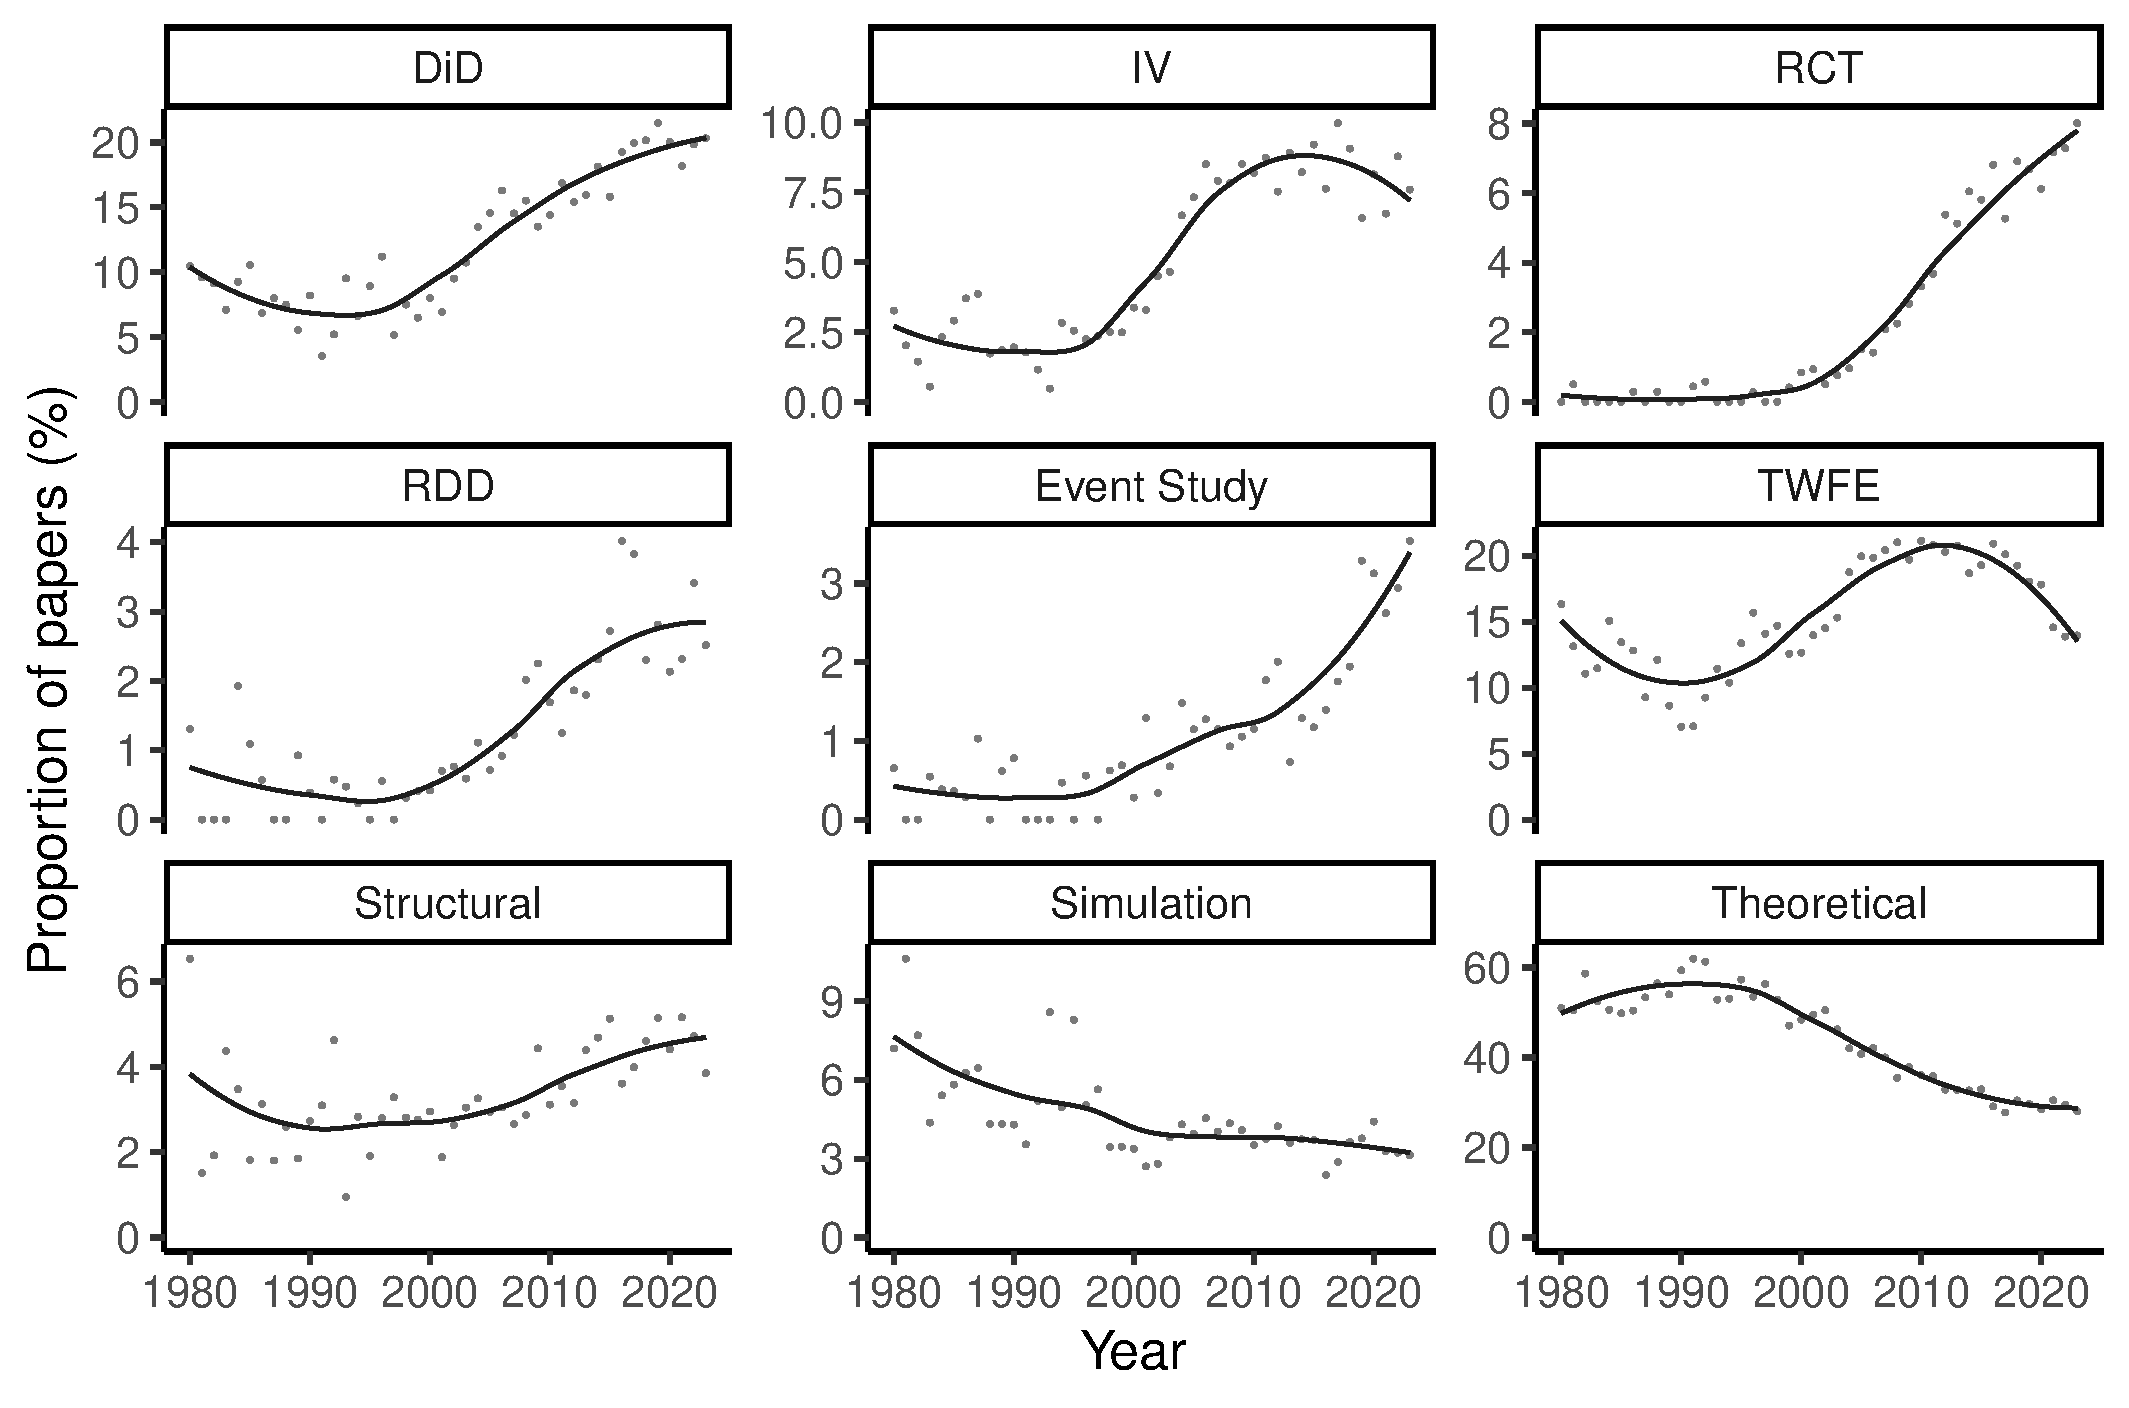
\includegraphics[width=0.84\linewidth,height=0.66\textheight,keepaspectratio]{proportion_papers_by_method_facet_plot.pdf}};
    \end{tikzpicture}
  \end{center}

  \figurecaptionbar{DiD, IV, and RCT rise, while theory-heavy papers become a smaller share of the working-paper universe.}
\end{frame}

\begin{frame}[t]{Fields still have very different method cultures}
  \begin{center}
    \begin{tikzpicture}
      \node[
        fill=white,
        draw=LineSoft,
        rounded corners=10pt,
        inner sep=6pt
      ] {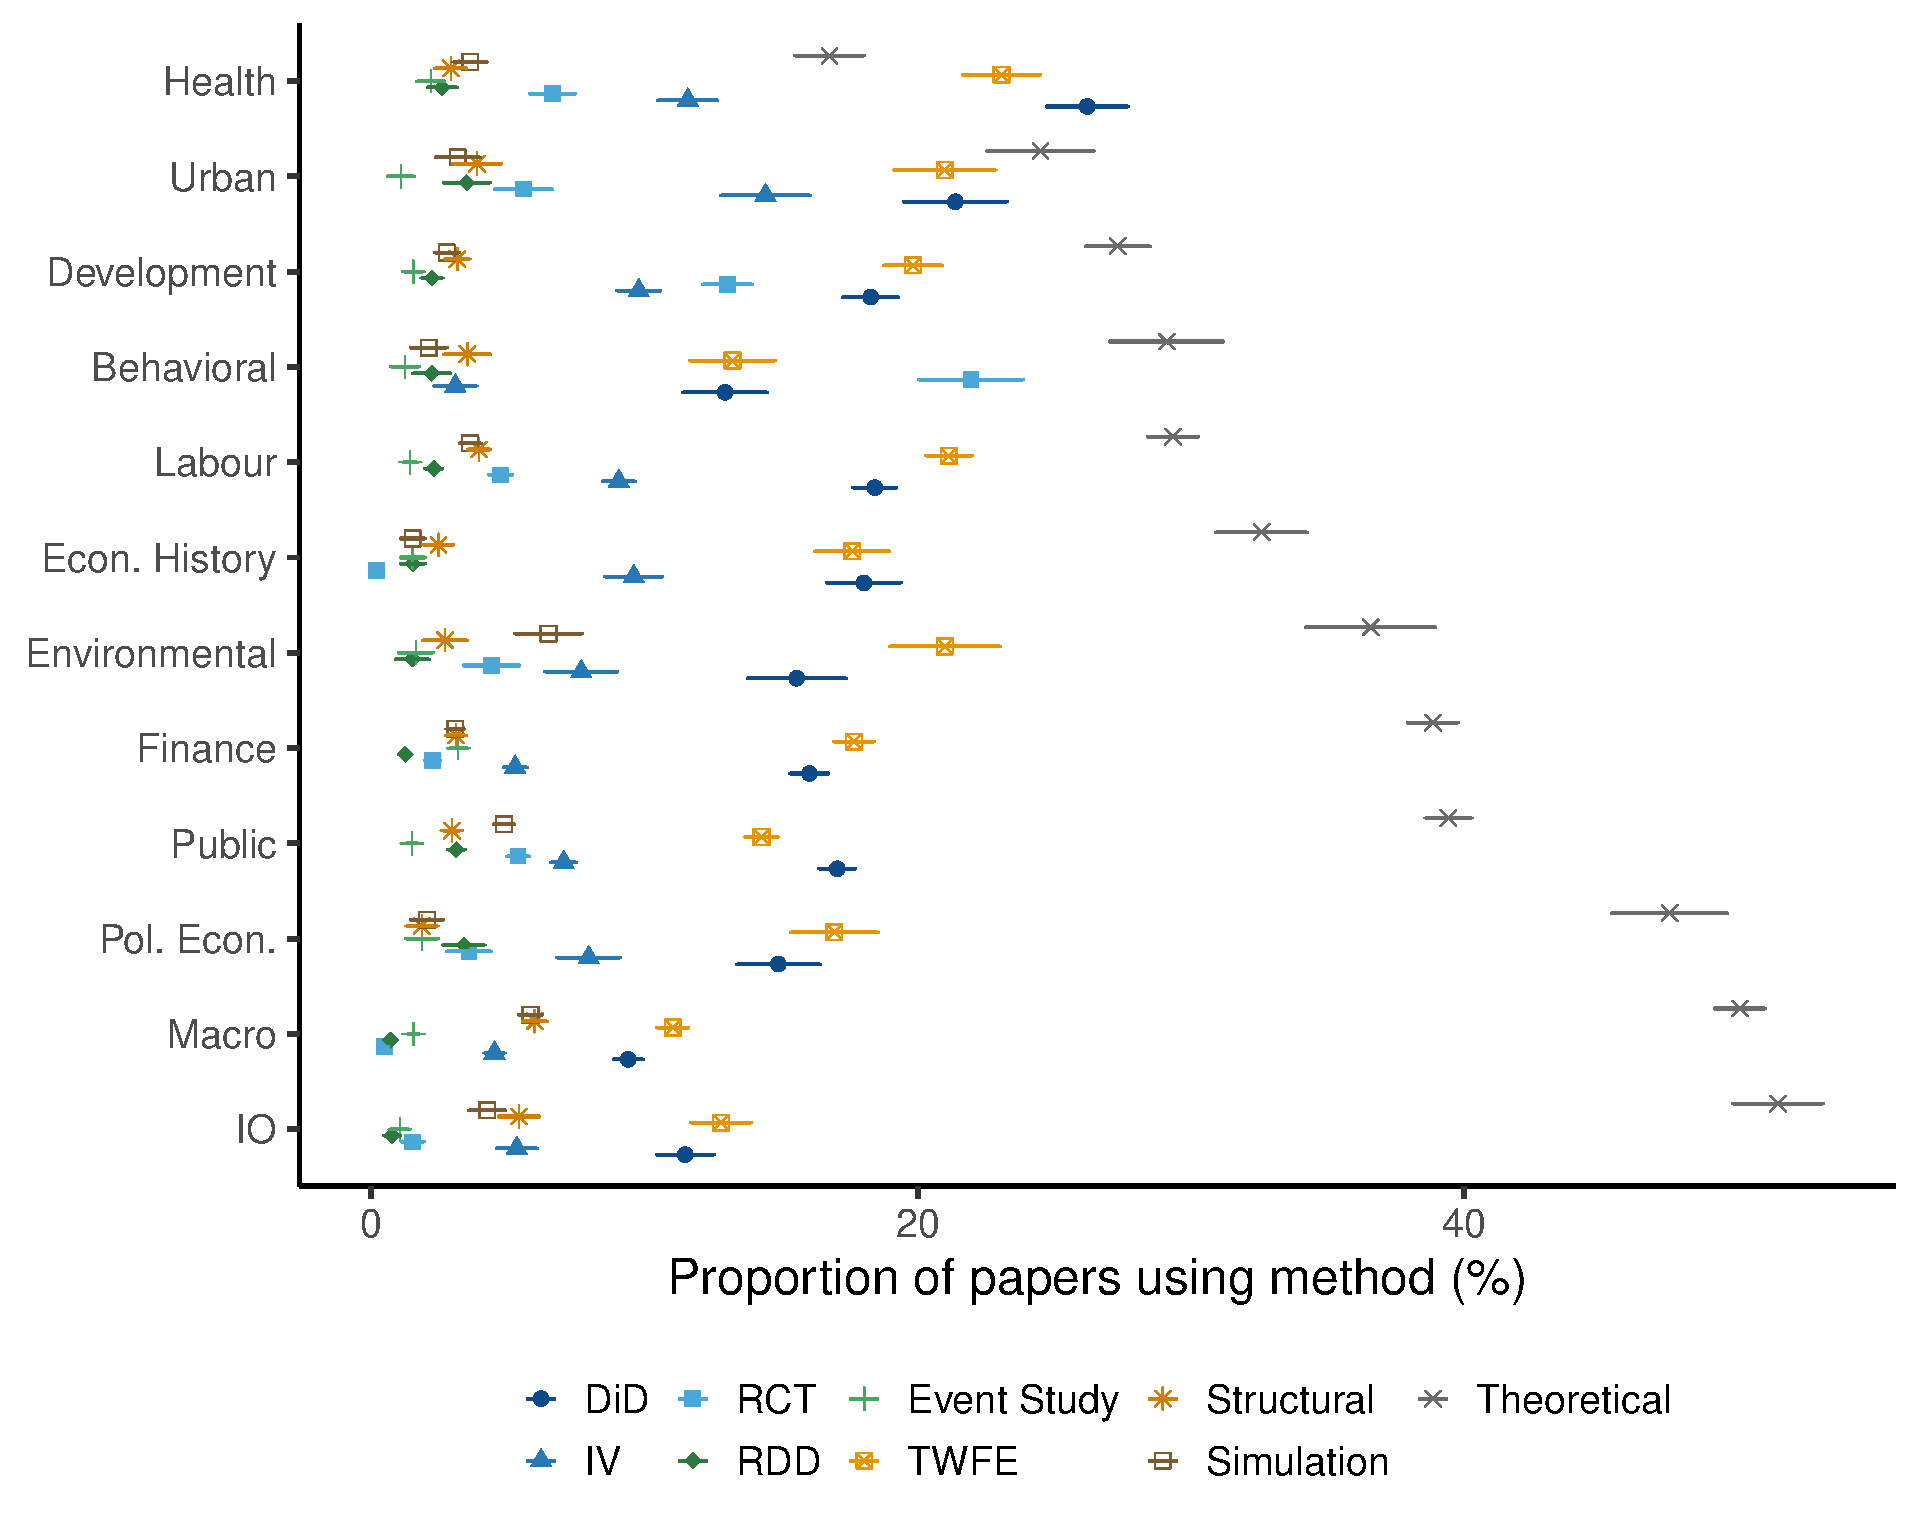
\includegraphics[width=0.82\linewidth,height=0.66\textheight,keepaspectratio]{method_usage_by_field_with_CI_and_mixed_methods.pdf}};
    \end{tikzpicture}
  \end{center}

  \figurecaptionbar{Method culture remains field-specific: DiD is strongest in urban/labour/public, RCTs in behavioral/development, and theory remains concentrated in macro, IO, and finance.}
\end{frame}

\BridgeSlide{}{Incentives}{What kinds of claim structures get rewarded?}

\section{What Gets Rewarded}

\SectionDivider{Incentives}{What gets rewarded}{Publication and citation patterns.}

\begin{frame}[t,label=main-measures]{Three families of paper-level measures}
  \begin{columns}[T,onlytextwidth]
    \begin{column}{0.31\textwidth}
      \only<1->{\Card{0.98\linewidth}{\MiniGraphComplexity\hfill Complexity}{
        How broad and deep is the argument?\par
        \smallskip
        Edges, unique paths, longest path}}
    \end{column}
    \begin{column}{0.31\textwidth}
      \only<2->{\Card{0.98\linewidth}{\MiniGraphNovelty\hfill Novelty}{
        Does the paper add genuinely new edges, paths, or gap-filling combinations?}}
    \end{column}
    \begin{column}{0.31\textwidth}
      \only<3->{\Card{0.98\linewidth}{\MiniGraphPosition\hfill Position}{
        Are the paper's concepts central, peripheral, or mixed inside the cumulative literature graph?}}
    \end{column}
  \end{columns}
\vspace{0.2cm}
\only<4->{\Card[PaperSand]{0.99\linewidth}{Main comparison}{
  Every family is computed in both \textcolor{CausalBlue}{causal} and \textcolor{NonCausalOrange}{non-causal} variants. That split is the paper's main empirical lever.}}
\end{frame}

\begin{frame}[t]{Which concepts stay central once we focus on causal edges?}
  \begin{center}
    \begin{tikzpicture}
      \node[
        fill=white,
        draw=LineSoft,
        rounded corners=10pt,
        inner sep=6pt
      ] {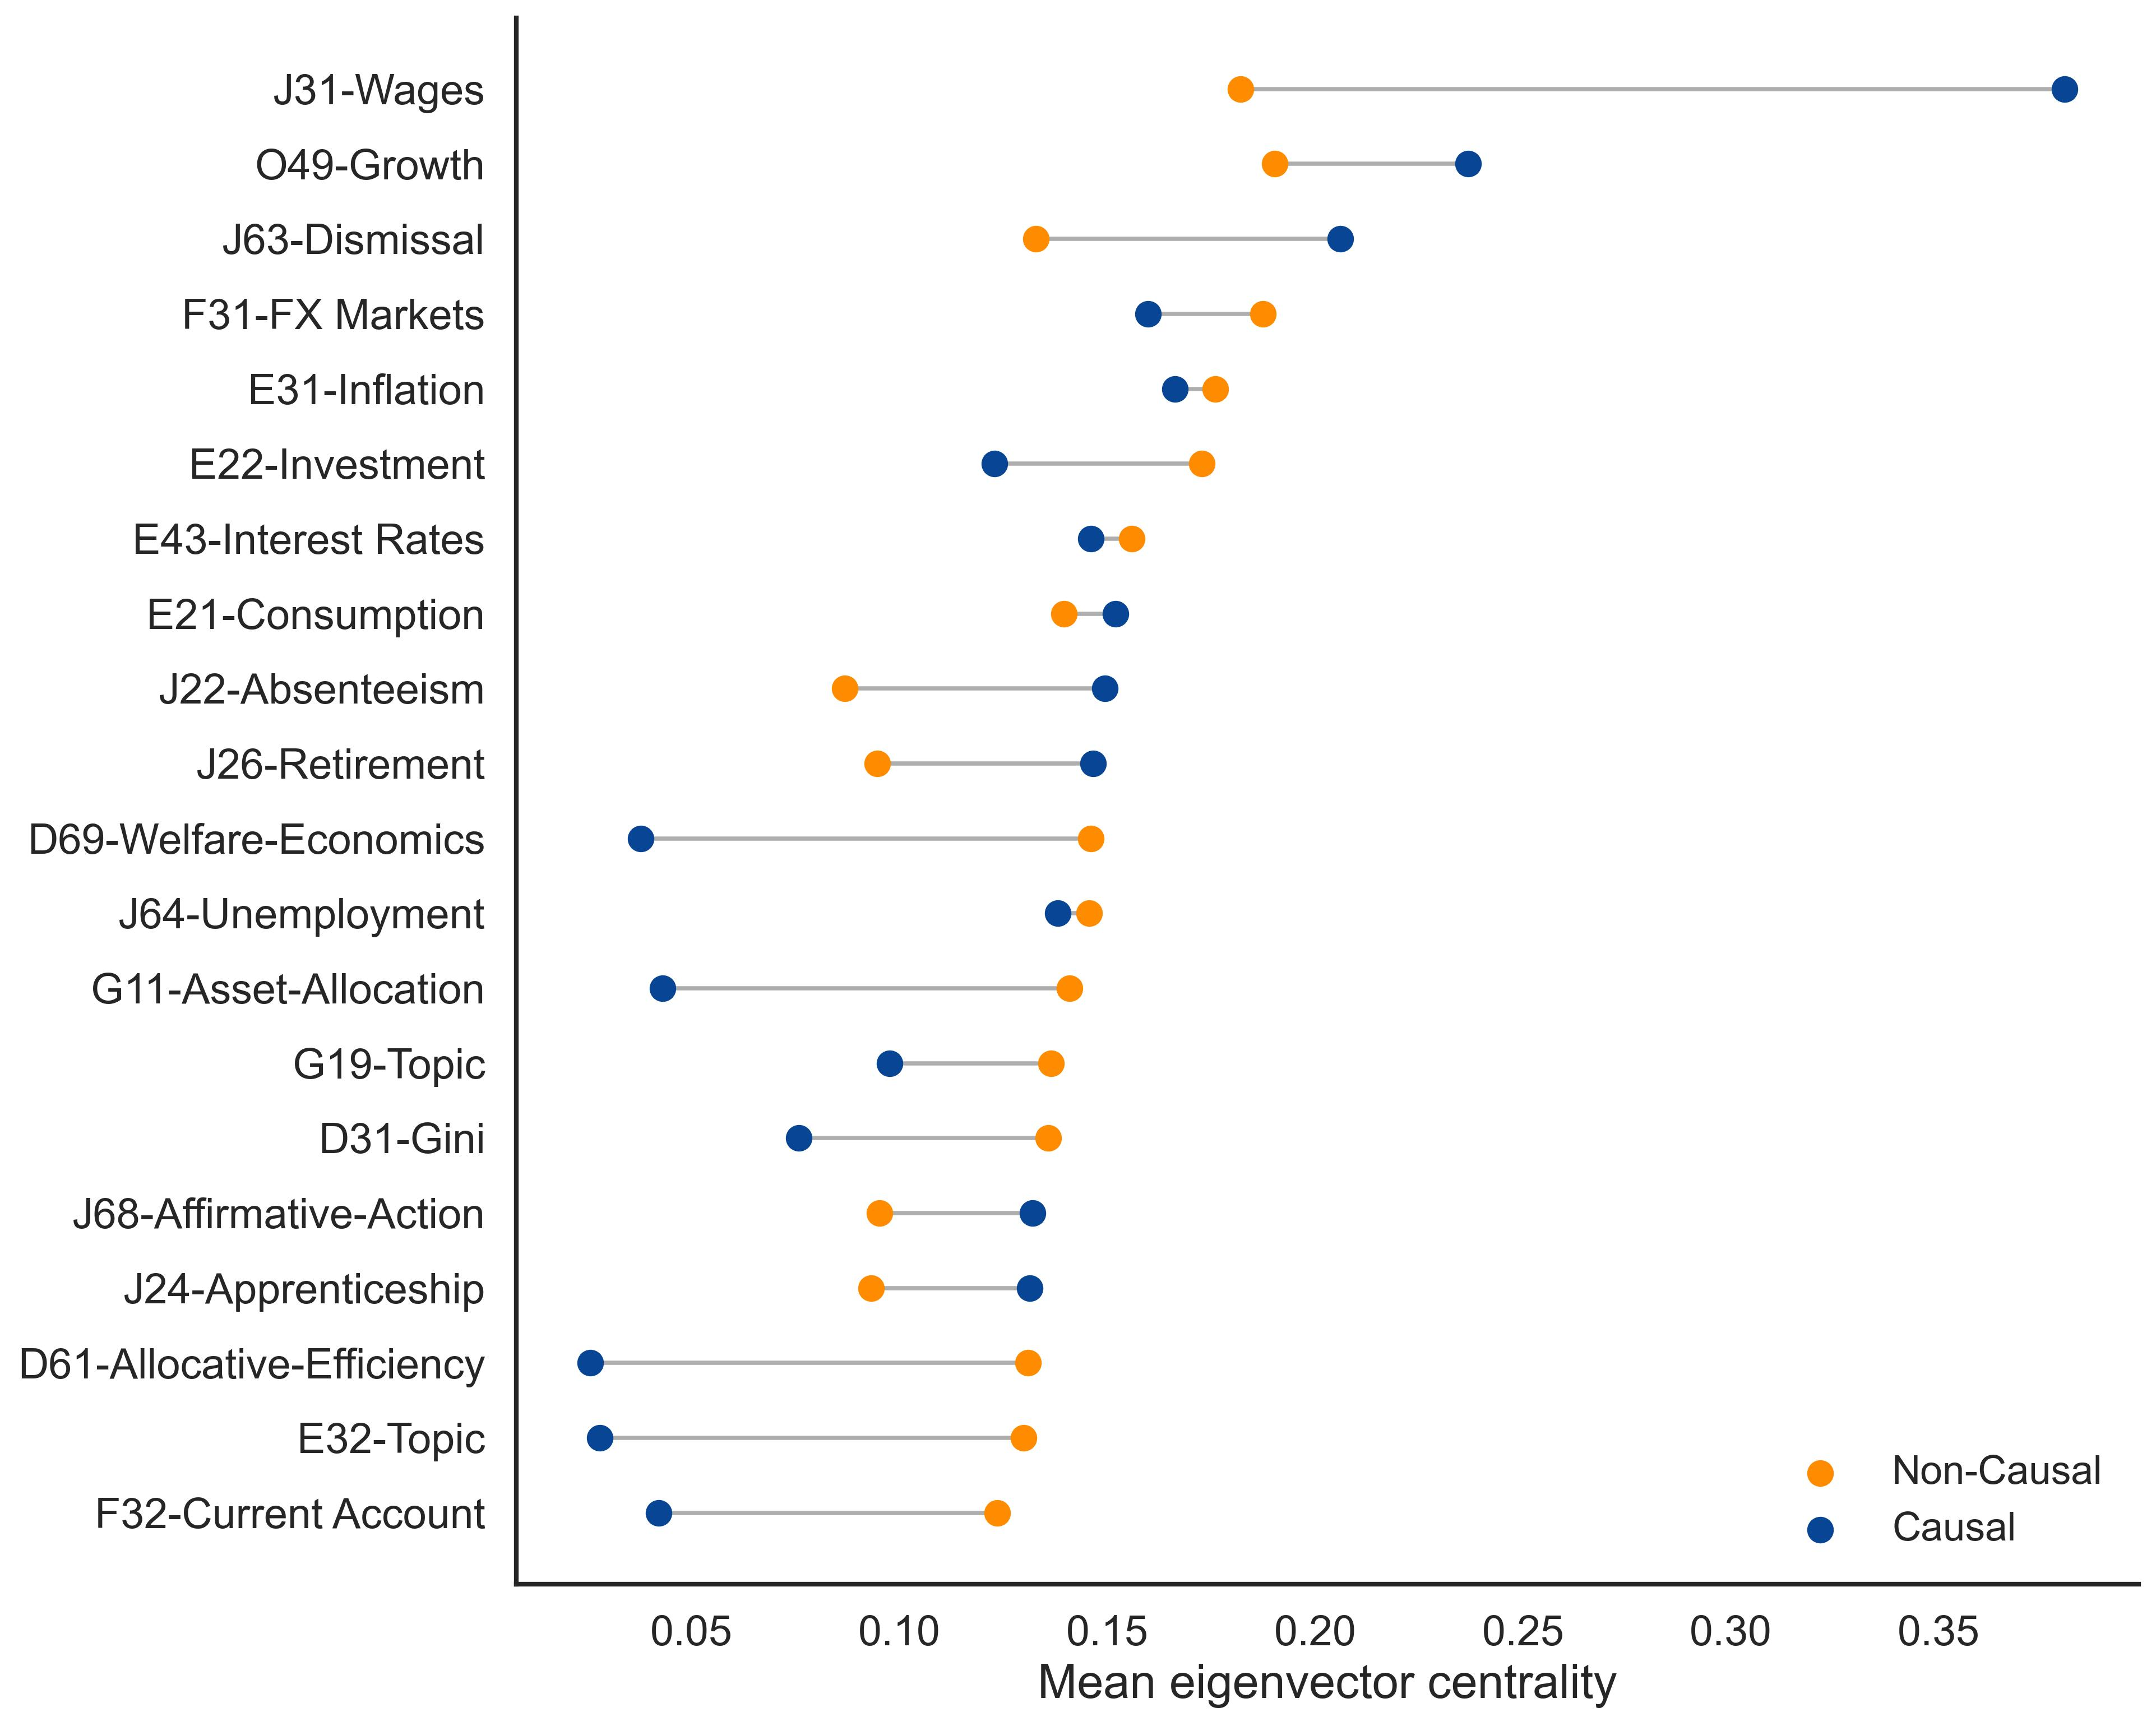
\includegraphics[width=0.76\linewidth,height=0.62\textheight,keepaspectratio]{top_20_jel_nodes_centrality_levels_appendix.jpg}};
    \end{tikzpicture}
  \end{center}
  \figurecaptionbar{Blue is causal centrality and orange is non-causal centrality. The x-axis is mean eigenvector centrality, not a regression coefficient.}
\end{frame}

\begin{frame}[t]{Concept centrality shifts once we focus on causal edges}
  \begin{center}
    \begin{tikzpicture}
      \node[
        fill=white,
        draw=LineSoft,
        rounded corners=10pt,
        inner sep=6pt
      ] {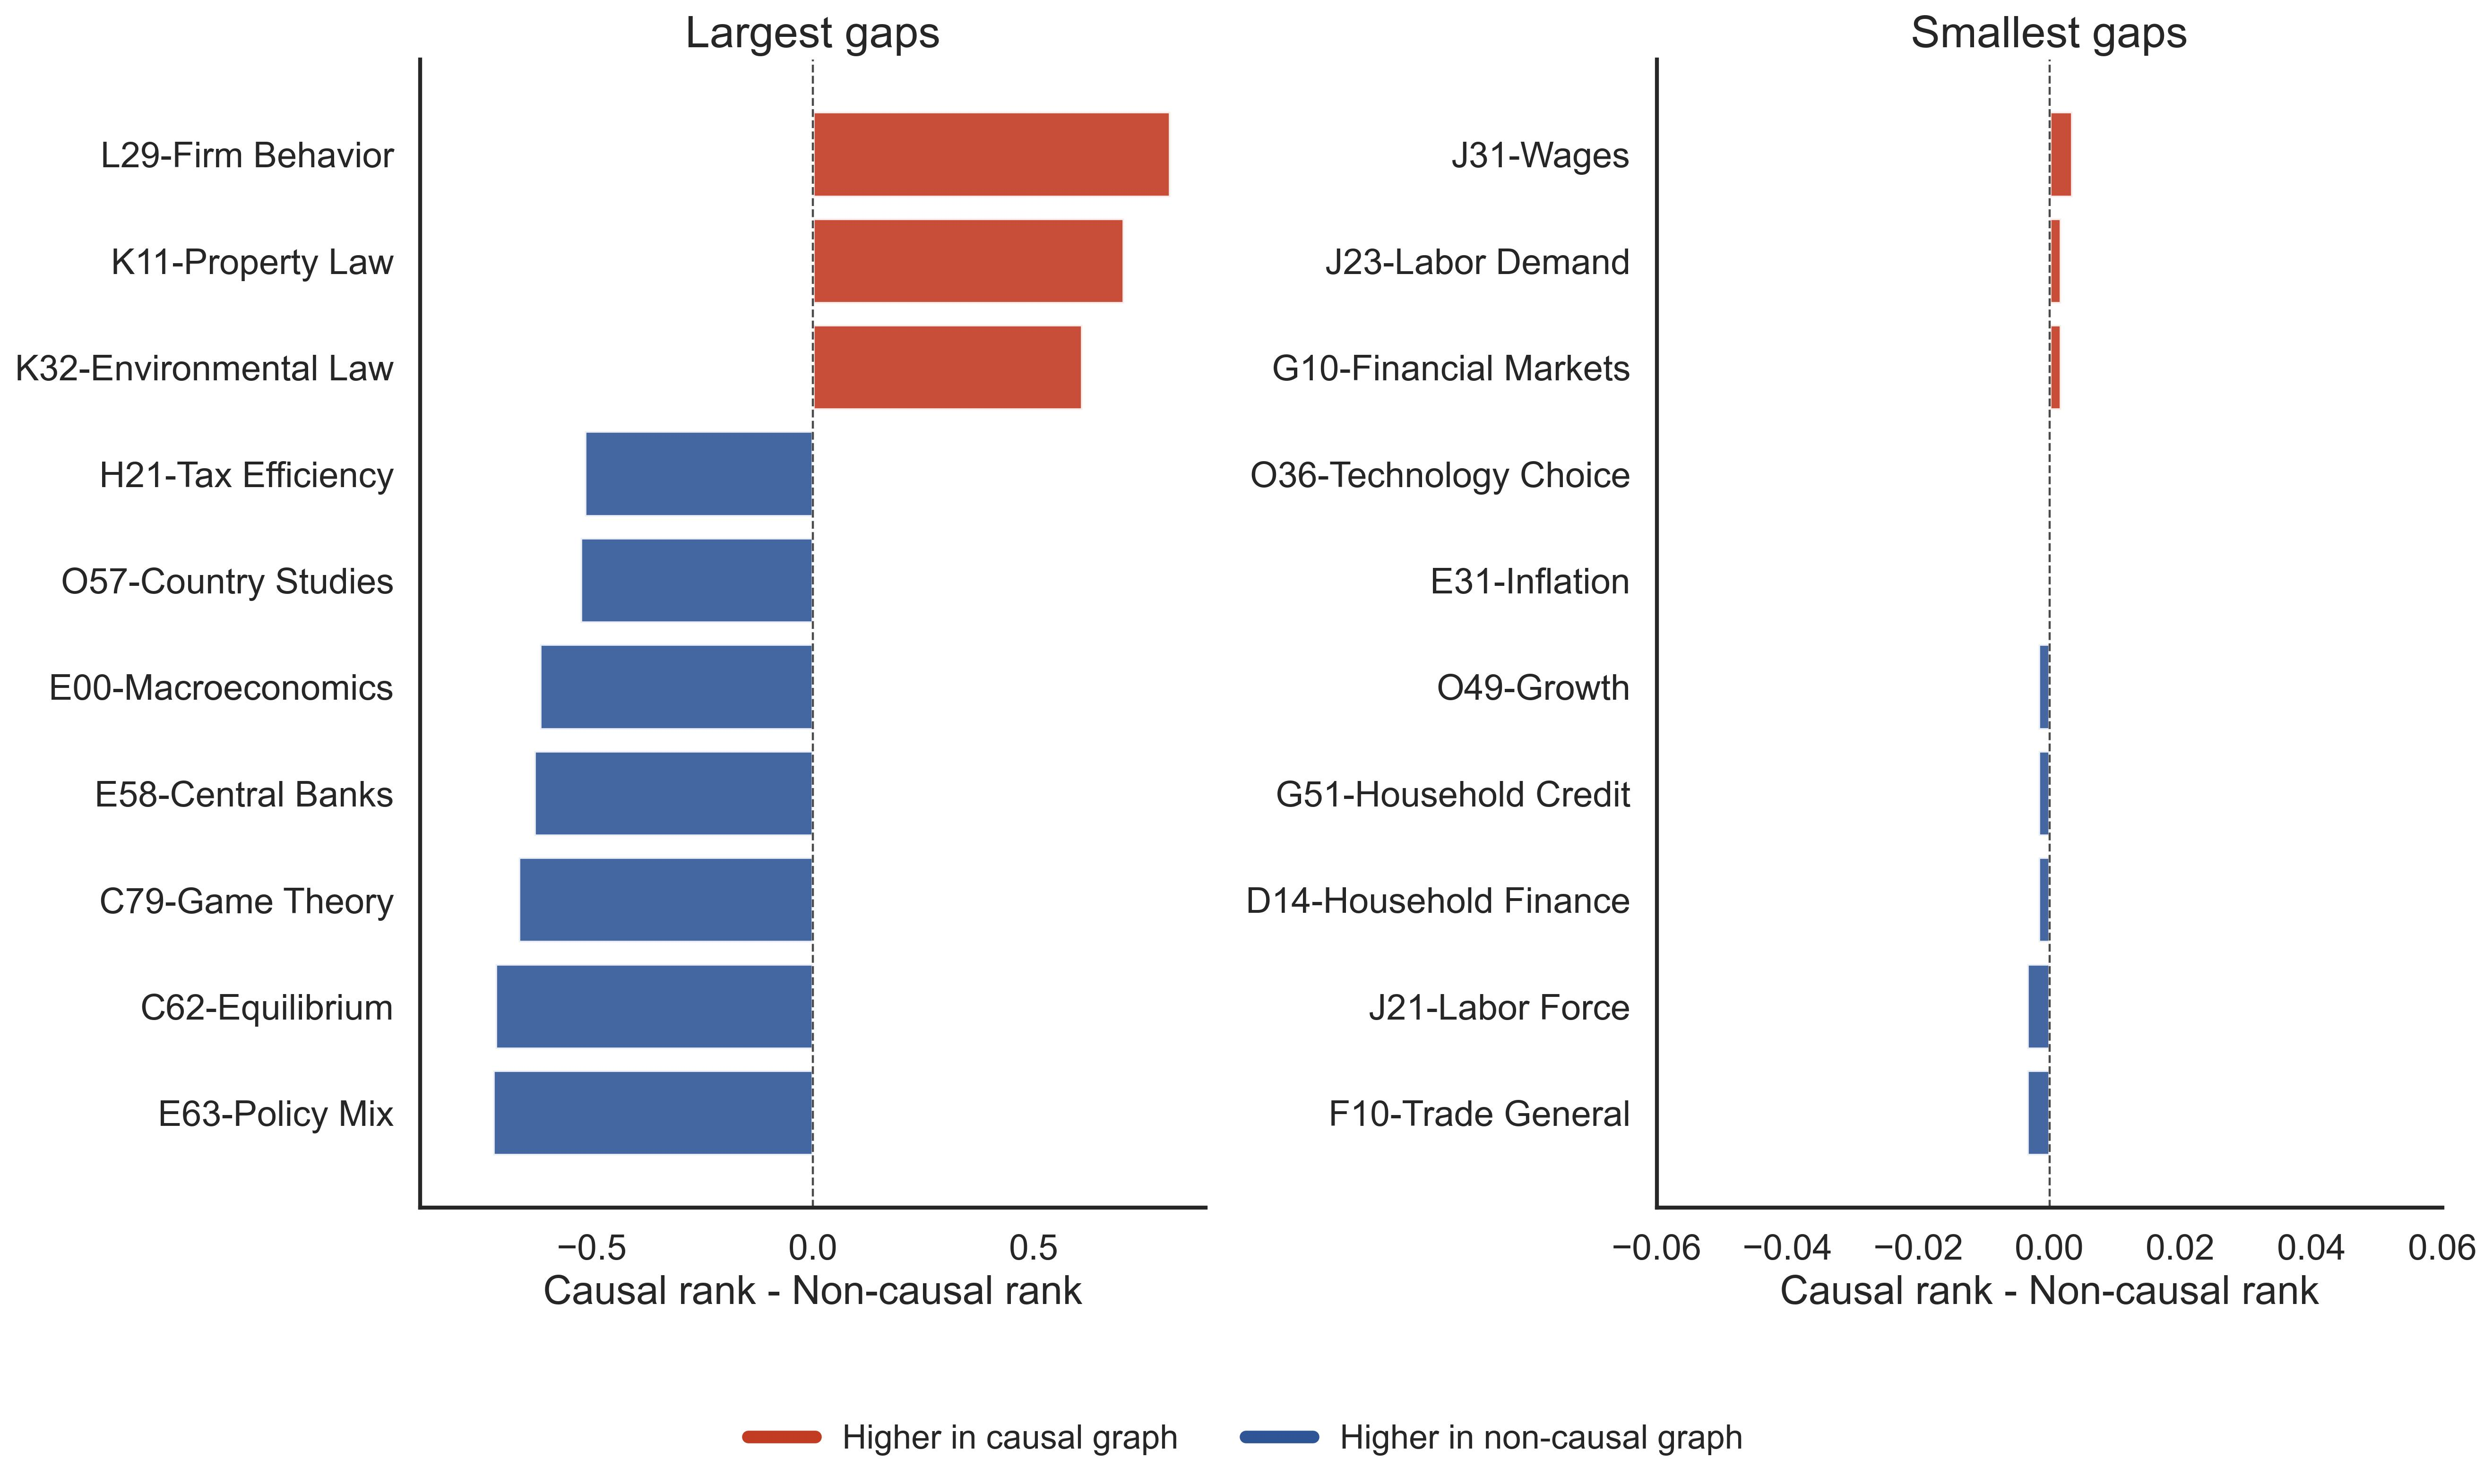
\includegraphics[width=0.78\linewidth,height=0.62\textheight,keepaspectratio]{top_20_jel_nodes_centrality_combined_non_causal.jpg}};
    \end{tikzpicture}
  \end{center}
  \figurecaptionbar{Some concepts move sharply up or down once the literature graph is restricted to causally identified edges.}
\end{frame}

\begin{frame}[t]{The empirical question is deliberately simple}
  \vspace{0.34cm}
  \begin{columns}[T,onlytextwidth]
    \begin{column}{0.36\textwidth}
      \begin{overlayarea}{\linewidth}{0.2\textheight}
      \only<1->{\Card{0.98\linewidth}{Outcome 1}{
        \textbf{Top journal placement}\par
        Top 5, 6--20, and 21--100 publication outcomes}}
      \end{overlayarea}

      \vspace{0.14cm}
      \begin{overlayarea}{\linewidth}{0.2\textheight}
      \only<2->{\Card{0.98\linewidth}{Outcome 2}{
        \textbf{Long-run influence}\par
        Log citations as of the September 2024 snapshot}}
      \end{overlayarea}
    \end{column}
    \begin{column}{0.6\textwidth}
      \begin{overlayarea}{\linewidth}{0.22\textheight}
      \only<3->{\Card[PaperSand]{0.98\linewidth}{Associational setup}{
        Regress each outcome on one graph measure with year fixed effects.\par\smallskip
        Then compare \textcolor{CausalBlue}{causal} and \textcolor{NonCausalOrange}{non-causal} versions of the same measure family.}}
      \end{overlayarea}

      \vspace{0.14cm}
      \begin{overlayarea}{\linewidth}{0.2\textheight}
      \only<4->{\Card[CausalBlue!7]{0.98\linewidth}{Hypothesis}{
        Papers with richer \textcolor{CausalBlue}{causal} structure and novelty should outperform papers whose extra structure is mostly non-causal.}}
      \end{overlayarea}
    \end{column}
  \end{columns}
\end{frame}

\begin{frame}[t,label=main-predictors]{Build the predictors result, one family at a time}
  \begin{tikzpicture}
    \node[inner sep=0,anchor=south west] (predfig) at (0,0) {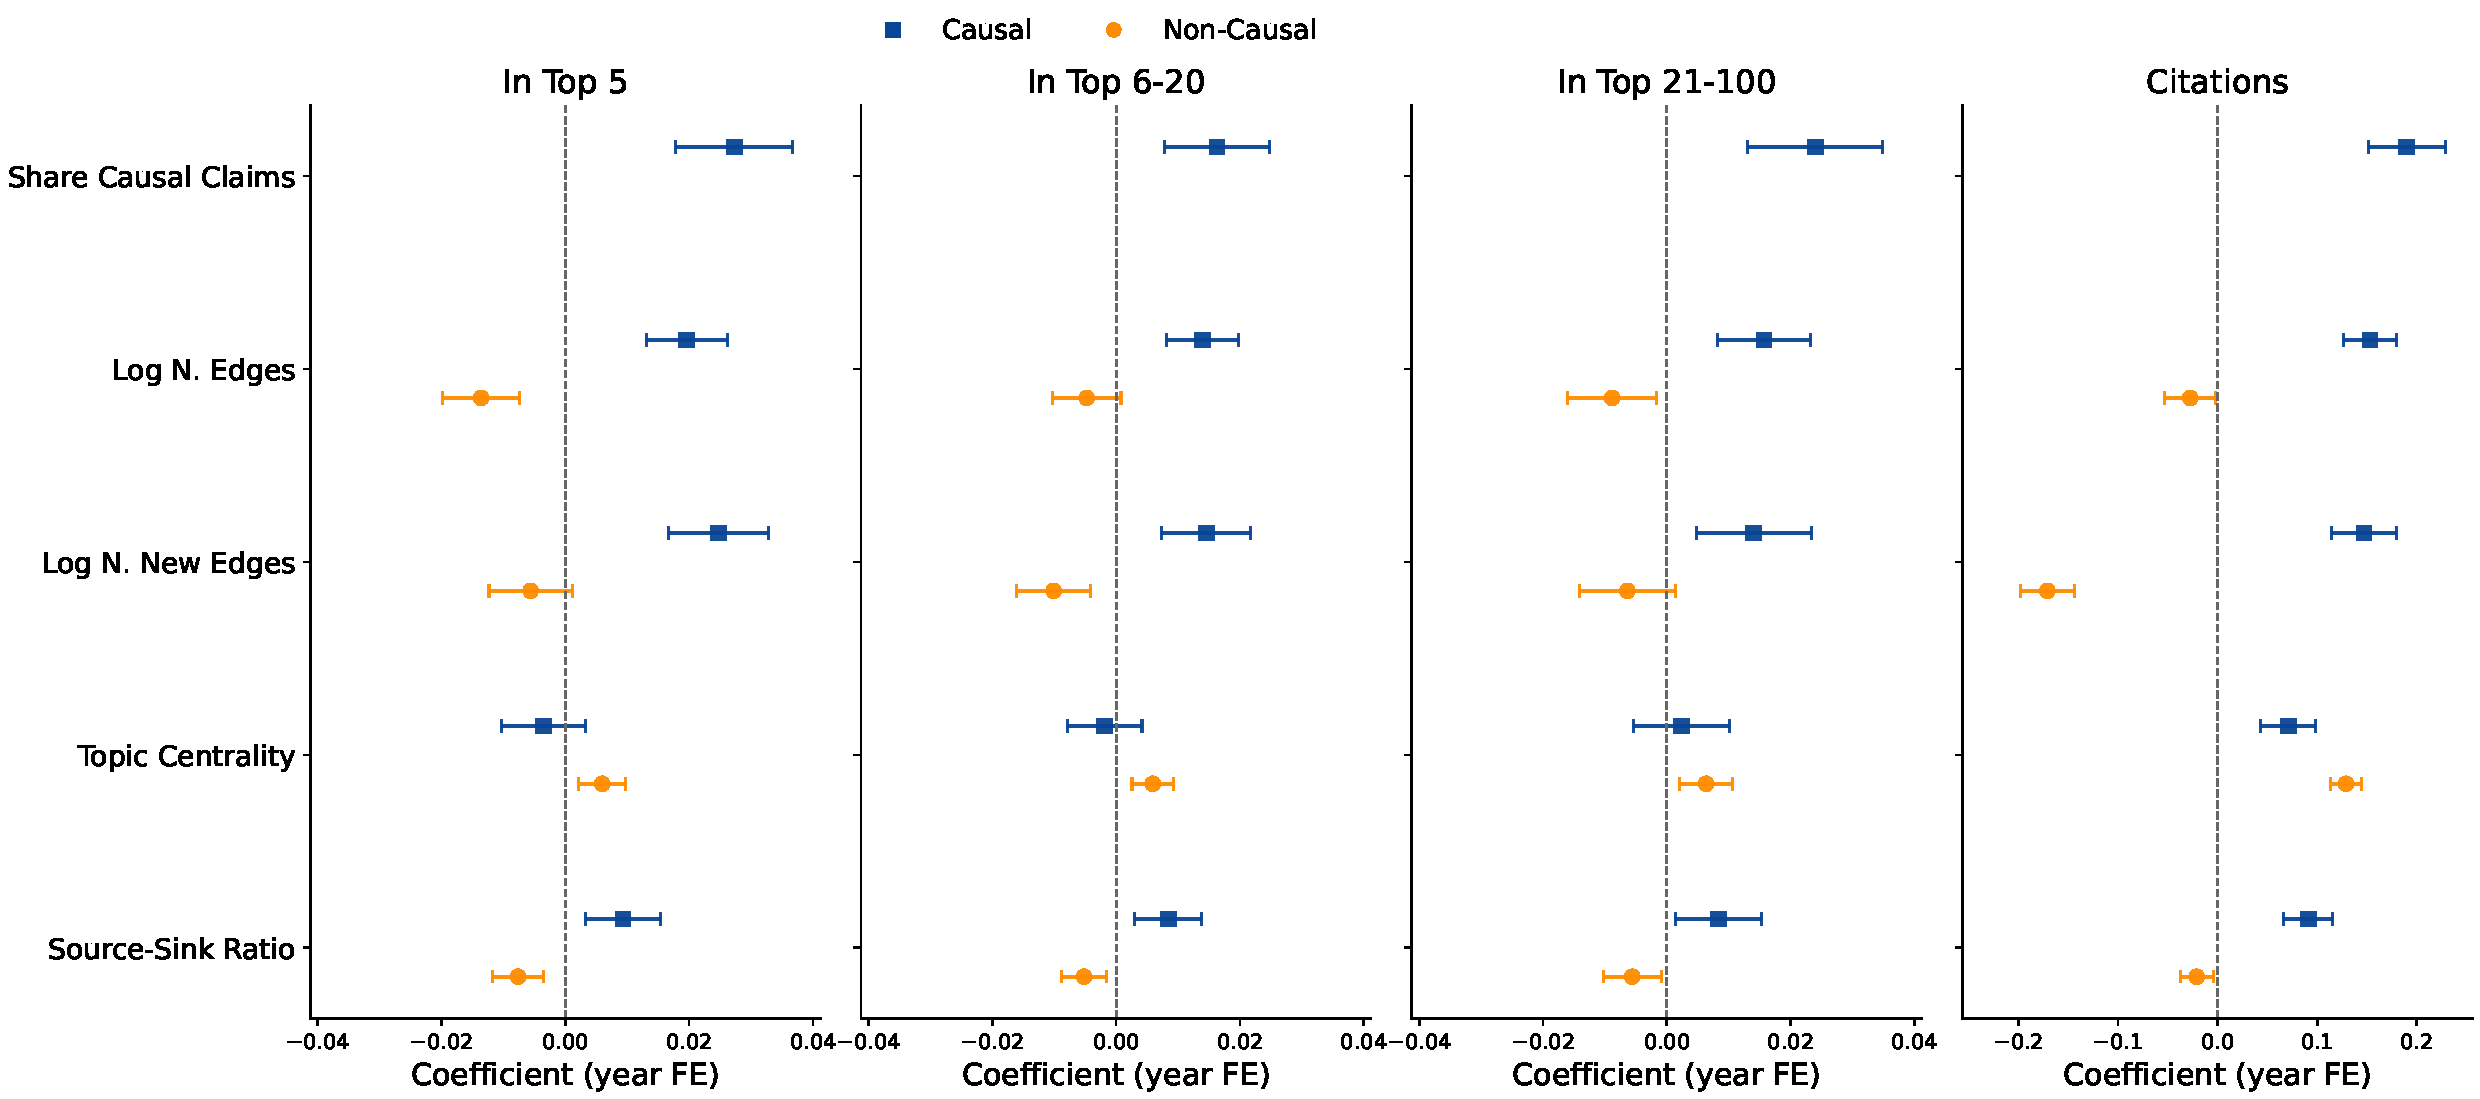
\includegraphics[width=0.95\linewidth]{publication_predictors_main_five_measures.pdf}};
    \begin{scope}[x={(predfig.south east)},y={(predfig.north west)}]
      \clip (0,0) rectangle (1,1);
      \foreach \y in {0.78,0.60,0.42,0.24}{
        \draw[Muted!35,dashed,line width=0.45pt] (0.15,\y) -- (0.995,\y);
      }

      \only<1>{
        \fill[white] (-0.025,0.06) rectangle (0.998,0.74);
      }
      \only<2>{
        \fill[white] (-0.025,0.06) rectangle (0.998,0.56);
      }
      \only<3>{
        \fill[white] (-0.025,0.06) rectangle (0.998,0.38);
      }
      \only<4>{
        \fill[white] (-0.025,0.06) rectangle (0.998,0.20);
      }
    \end{scope}
  \end{tikzpicture}

  \vspace{0.15cm}
  \only<1>{\PredictorStrip{CausalBlue}{1. Causal share}{Higher causal share improves placement and citations.}}

  \only<2>{\PredictorStrip{CausalBlue}{2. Complexity}{More \textcolor{CausalBlue}{causal} edges help; the non-causal analogue does not.}}

  \only<3>{\PredictorStrip{CausalBlue}{3. Novelty}{New \textcolor{CausalBlue}{causal} edges predict payoff; new non-causal edges do not.}}

  \only<4>{\PredictorStrip{AccentTeal}{4. Centrality}{Centrality helps citations more than editorial selection.}}

  \only<5->{\PredictorStrip{CausalBlue}{5. Source-heavy}{Source-heavy \textcolor{CausalBlue}{causal} structure is rewarded; non-causal is not.}}

  \vspace{0.08cm}
  \hfill\JumpButton{app-predictor-variants}{Variant measures}
\end{frame}

\begin{frame}[t]{Selection and diffusion are not the same game}
  \begin{columns}[T,onlytextwidth]
    \begin{column}{0.46\textwidth}
      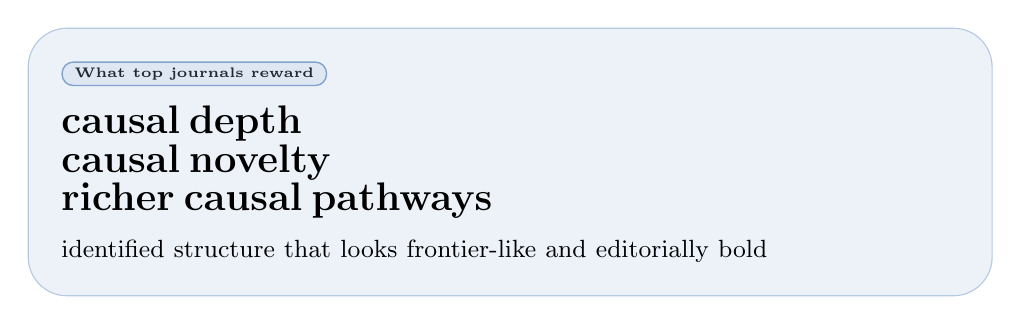
\begin{tikzpicture}
        \node[
          fill=CausalBlue!8,
          draw=CausalBlue!32,
          rounded corners=14pt,
          inner sep=12pt,
          text width=0.94\linewidth,
          align=left
        ] {\chip[CausalBlue]{What top journals reward}\par
          \vspace{0.22cm}
          {\Large\bfseries causal depth}\par
          {\Large\bfseries causal novelty}\par
          {\Large\bfseries richer causal pathways}\par
          \vspace{0.18cm}
          \small identified structure that looks frontier-like and editorially bold};
      \end{tikzpicture}
    \end{column}
    \begin{column}{0.08\textwidth}
      \vspace{1.35cm}
      \centering
      {\fontsize{22}{24}\selectfont\bfseries\textcolor{AccentCoral}{vs.}}
    \end{column}
    \begin{column}{0.46\textwidth}
      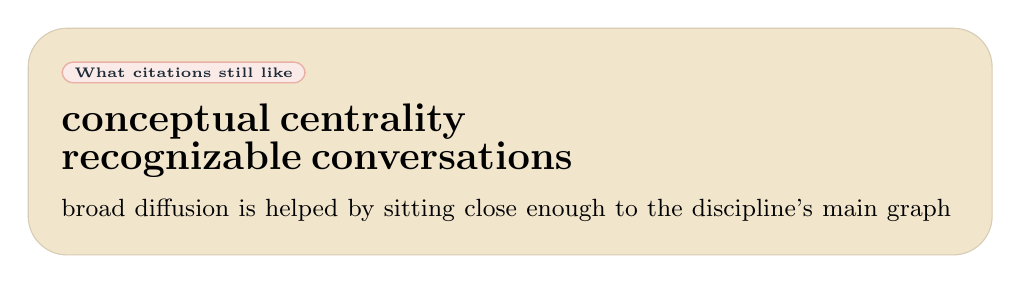
\begin{tikzpicture}
        \node[
          fill=PaperSand,
          draw=LineSoft,
          rounded corners=14pt,
          inner sep=12pt,
          text width=0.94\linewidth,
          align=left
        ] {\chip[AccentCoral]{What citations still like}\par
          \vspace{0.22cm}
          {\Large\bfseries conceptual centrality}\par
          {\Large\bfseries recognizable conversations}\par
          \vspace{0.18cm}
          \small broad diffusion is helped by sitting close enough to the discipline's main graph};
      \end{tikzpicture}
    \end{column}
  \end{columns}

  \vspace{0.28cm}
  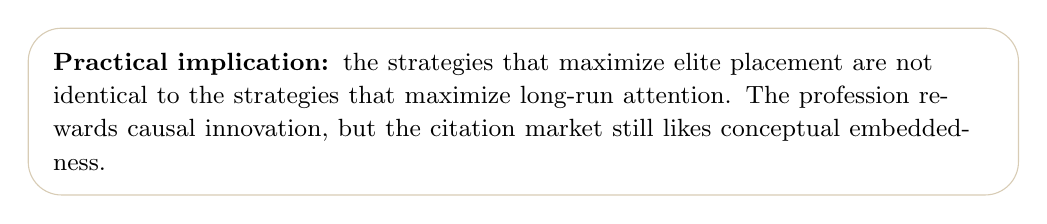
\begin{tikzpicture}
    \node[
      fill=white,
      draw=LineSoft,
      rounded corners=12pt,
      inner sep=9pt,
      text width=0.985\linewidth,
      align=left
    ] {\small\textbf{Practical implication:} the strategies that maximize elite placement are not identical to the strategies that maximize long-run attention. The profession rewards causal innovation, but the citation market still likes conceptual embeddedness.};
  \end{tikzpicture}
\end{frame}

\begin{frame}[t]{What this still does not do}
  \begin{columns}[T,onlytextwidth]
    \begin{column}{0.32\textwidth}
      
\begin{tikzpicture}
        \node[
          fill=white,
          draw=LineSoft,
          rounded corners=12pt,
          inner sep=8pt,
          text width=0.9\linewidth,
          align=left
        ] (limone) {\chip[AccentCoral]{1. Truth}\par
          \vspace{0.08cm}
          \textbf{No truth test.}\par
          \footnotesize Records stated claims, not correctness.};
        \fill[AccentCoral] ([xshift=0.02cm]limone.north west) rectangle ([xshift=0.18cm]limone.south west);
      \end{tikzpicture}
    \end{column}
    \begin{column}{0.32\textwidth}
      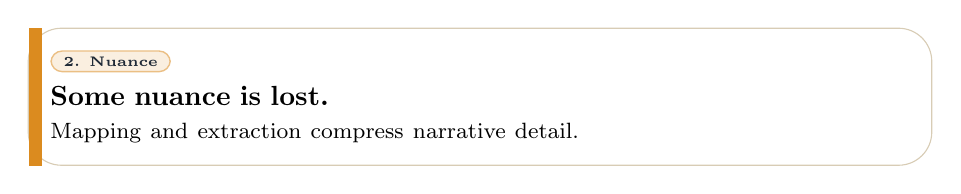
\begin{tikzpicture}
        \node[
          fill=white,
          draw=LineSoft,
          rounded corners=12pt,
          inner sep=8pt,
          text width=0.9\linewidth,
          align=left
        ] (limtwo) {\chip[NonCausalOrange]{2. Nuance}\par
          \vspace{0.08cm}
          \textbf{Some nuance is lost.}\par
          \footnotesize Mapping and extraction compress narrative detail.};
        \fill[NonCausalOrange] ([xshift=0.02cm]limtwo.north west) rectangle ([xshift=0.18cm]limtwo.south west);
      \end{tikzpicture}
    \end{column}
    \begin{column}{0.32\textwidth}
      
\begin{tikzpicture}
        \node[
          fill=white,
          draw=LineSoft,
          rounded corners=12pt,
          inner sep=8pt,
          text width=0.9\linewidth,
          align=left
        ] (limthree) {\chip[AccentTeal]{3. Scope}\par
          \vspace{0.08cm}
          \textbf{The window is fixed.}\par
          \footnotesize The 30-page window can miss later detail.};
        \fill[AccentTeal] ([xshift=0.02cm]limthree.north west) rectangle ([xshift=0.18cm]limthree.south west);
      \end{tikzpicture}
    \end{column}
  \end{columns}

  \vspace{0.22cm}
  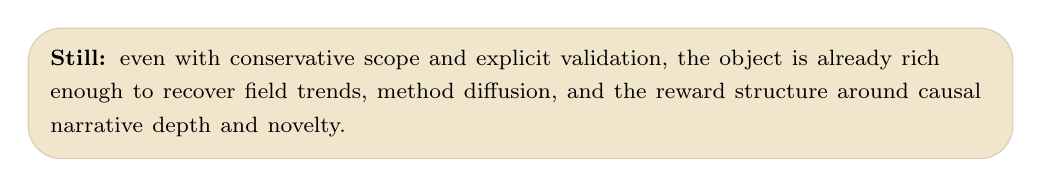
\begin{tikzpicture}
    \node[
      fill=PaperSand,
      draw=LineSoft,
      rounded corners=12pt,
      inner sep=8pt,
      text width=0.985\linewidth,
      align=left
    ] {\footnotesize\textbf{Still:} even with conservative scope and explicit validation, the object is already rich enough to recover field trends, method diffusion, and the reward structure around causal narrative depth and novelty.};
  \end{tikzpicture}
\end{frame}

\begin{frame}[plain]
  \begin{tikzpicture}[remember picture,overlay]
    \fill[AccentTeal!12] (current page.south west) rectangle (current page.north east);
    \fill[PaperCard] ([xshift=0.75cm,yshift=0.85cm]current page.south west) rectangle ([xshift=-0.75cm,yshift=-0.85cm]current page.north east);
    \draw[LineSoft,line width=0.8pt] ([xshift=0.75cm,yshift=0.85cm]current page.south west) rectangle ([xshift=-0.75cm,yshift=-0.85cm]current page.north east);
  \end{tikzpicture}

  \vspace{0.8cm}
  \chip[CausalBlue]{Closing}
  \vspace{0.22cm}

  {\fontsize{24}{28}\selectfont\bfseries Claim graphs turn papers into queryable objects.\par}
  \vspace{0.18cm}

  {\normalsize\textcolor{Muted}{That makes literatures easier to compare, aggregate, and extend.}\par}

  \vfill
  {\small\href{https://www.causal.claims}{\textbf{\textcolor{CausalBlue}{causal.claims}}}\par}
\end{frame}

\appendix
\section{Appendix}

\SectionDivider{Appendix}{Robustness, validation, and extra visuals}{Optional slides for discussion and follow-up questions.}

\begin{frame}[t,label=app-eo-trend]{EO robustness: the causal-edge trend is not a threshold artifact}
  \hfill\BackButton{main-trend}\par
  \vspace{0.08cm}
  \begin{tikzpicture}
    \node[
      fill=white,
      draw=LineSoft,
      rounded corners=10pt,
      inner sep=6pt
    ] {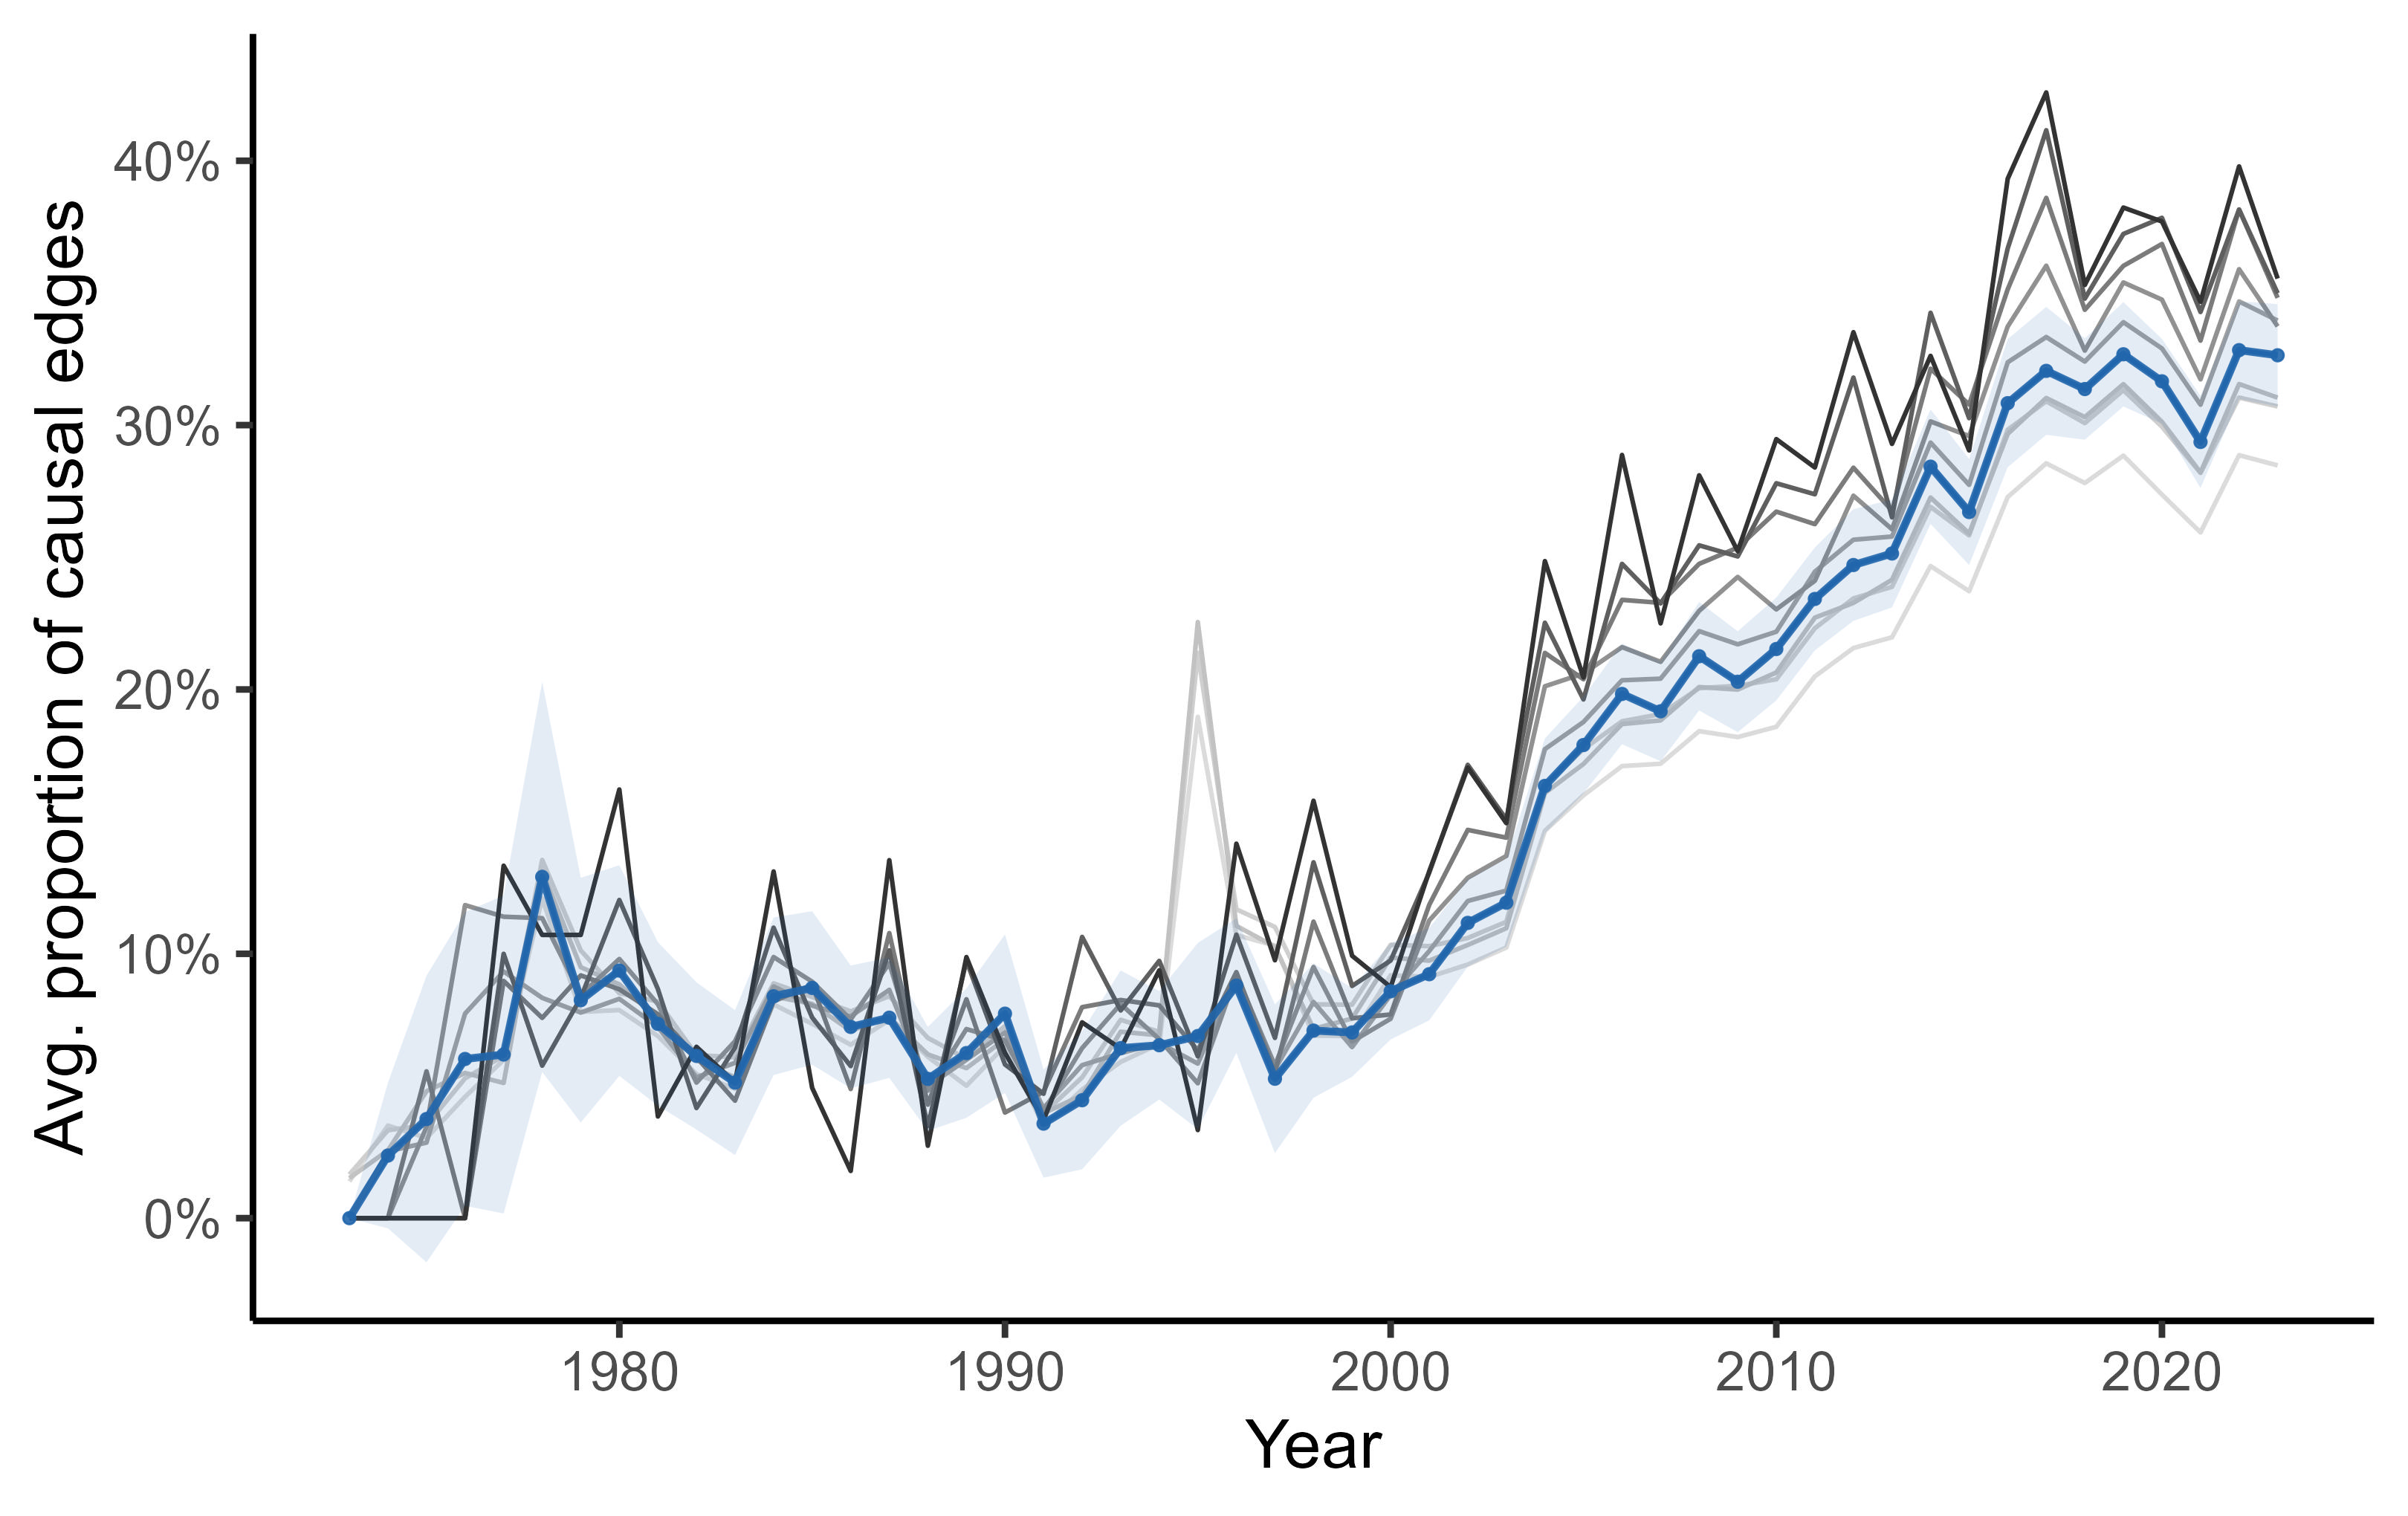
\includegraphics[width=0.88\linewidth,height=0.68\textheight,keepaspectratio]{prop_causal_edges_ts_overlay.jpg}};
  \end{tikzpicture}
  \figurecaptionbar{The rise in causal-edge share is preserved as EO gets stricter; the paper's baseline of EO >= 4 is a conservative but not extreme operating point.}
\end{frame}

\begin{frame}[t,label=app-eo-reg]{EO robustness: headline regression signs remain stable}
  \hfill\BackButton{main-predictors}\par
  \vspace{0.08cm}
  \begin{columns}[T,onlytextwidth]
    \begin{column}{0.78\textwidth}
      \begin{tikzpicture}
        \node[
          fill=white,
          draw=LineSoft,
          rounded corners=10pt,
          inner sep=6pt
        ] {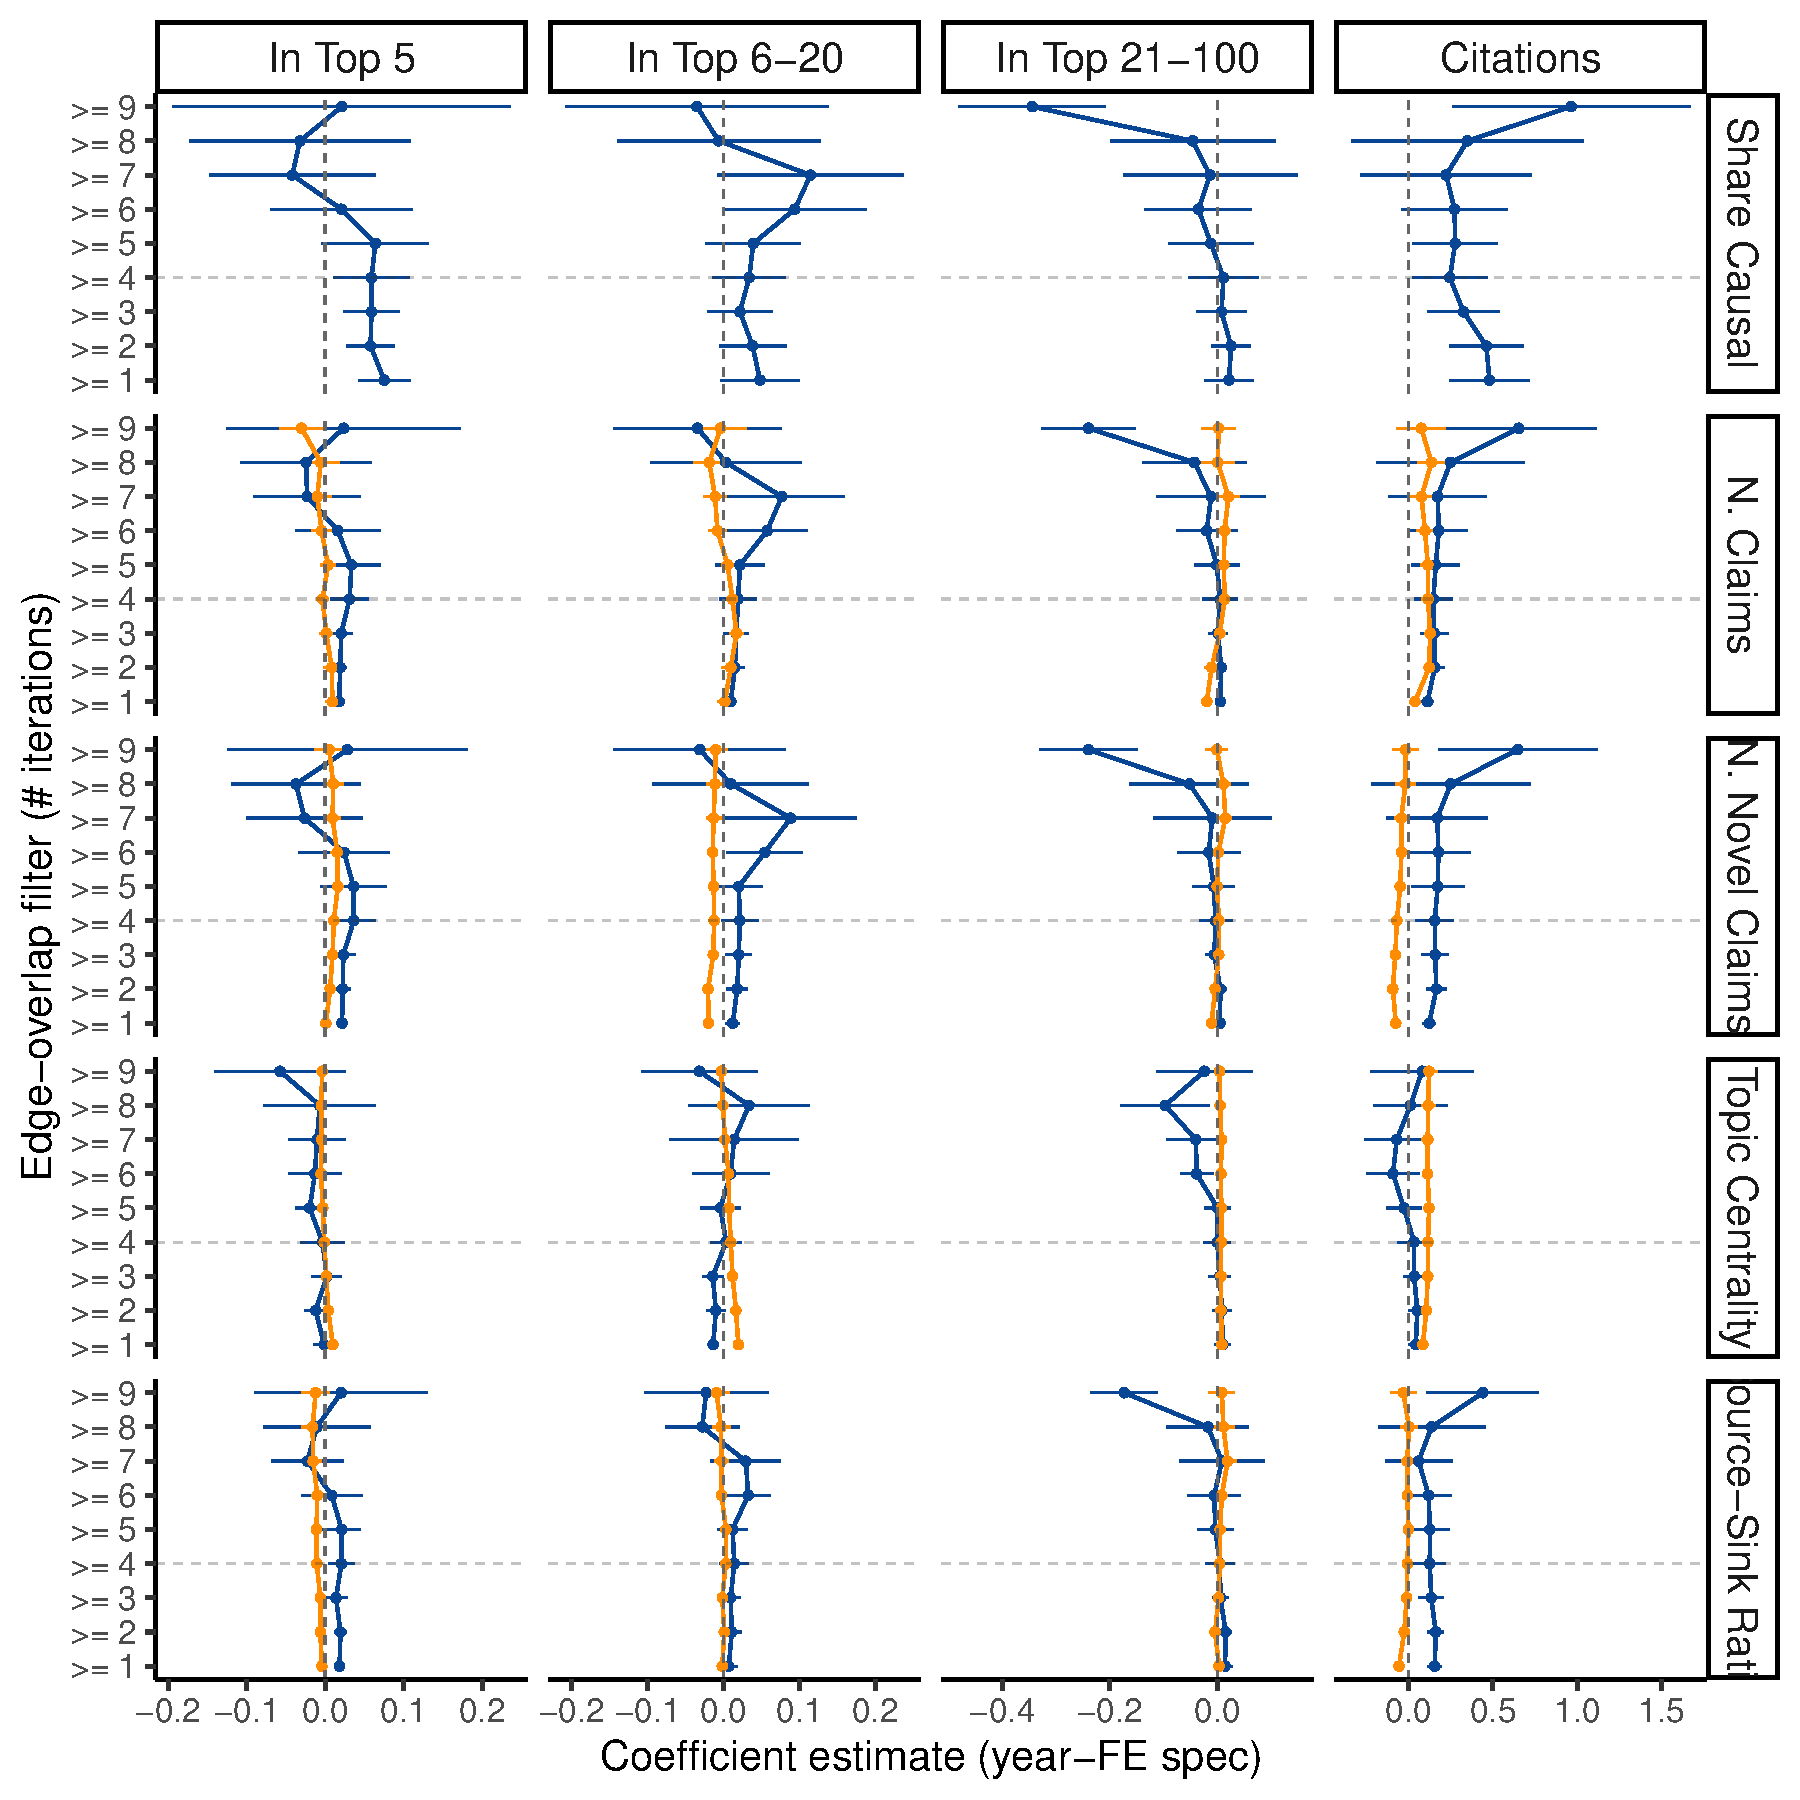
\includegraphics[width=0.98\linewidth,height=0.69\textheight,keepaspectratio]{main_reg_edge_overlap_grid.pdf}};
      \end{tikzpicture}
    \end{column}
    \begin{column}{0.18\textwidth}
      \vspace{0.9cm}
      \Card[PaperSand]{0.95\linewidth}{Takeaway}{
        Signs are stable through EO >= 4.\par\smallskip
        Intervals widen only once support becomes very thin.}
    \end{column}
  \end{columns}
\end{frame}

\begin{frame}[t,label=app-brodeur]{Validation: Brodeur benchmark}
  \hfill\BackButton{main-validation}\par
  \vspace{0.08cm}
  \Card[PaperSand]{0.99\linewidth}{Matched sample sizes}{
    EO >= 4: 285 papers \hspace{1em} EO >= 7: 169 papers \hspace{1em} EO = 9: 90 papers}

  \vspace{0.14cm}
  \begin{columns}[T,onlytextwidth]
    \begin{column}{0.48\textwidth}
      \Card{0.98\linewidth}{Method recovery}{
        Explicit quasi-experimental designs are recovered well in matched papers, especially for IV and for the cleaner DiD and RDD cases.}
    \end{column}
    \begin{column}{0.48\textwidth}
      \Card[CausalBlue!7]{0.98\linewidth}{Threshold pattern}{
        Raising the EO threshold improves precision, but support thins out as we keep only the most strongly backed edges.}
    \end{column}
  \end{columns}

  \vspace{0.18cm}
  \Card[white]{0.99\linewidth}{Why this matters}{
    This external benchmark suggests the pipeline is not just finding economics words; it is recovering recognizable causal-design labels.}
  \figurecaptionbar{The validation target here is recognizable method labeling, not full causal adjudication.}
\end{frame}

\begin{frame}[t,label=app-plausibly]{Validation: Plausibly Exogenous benchmark}
  \hfill\BackButton{main-validation}\par
  \vspace{0.08cm}
  \Card[PaperSand]{0.99\linewidth}{Matched sample sizes}{
    EO >= 4: 491 papers \hspace{1em} EO >= 7: 296 papers \hspace{1em} EO = 9: 148 papers}

  \vspace{0.14cm}
  \begin{columns}[T,onlytextwidth]
    \begin{column}{0.48\textwidth}
      \Card{0.98\linewidth}{Semantic alignment}{
        Retrieved snippets line up meaningfully with the cause, effect, and exogenous-variation language in the benchmark corpus.}
    \end{column}
    \begin{column}{0.48\textwidth}
      \Card[CausalBlue!7]{0.98\linewidth}{Strongest signal}{
        Exogenous variation is the cleanest component across thresholds, which is exactly the part we most want to isolate in causal claims.}
    \end{column}
  \end{columns}

  \vspace{0.18cm}
  \Card[white]{0.99\linewidth}{Why this matters}{
    The pipeline is not only tagging designs; it is also finding the semantic content around the shock or variation that identifies the claim.}
  \figurecaptionbar{The strongest semantic lift comes from text describing exogenous variation.}
\end{frame}

\begin{frame}[t,label=app-snippet]{Validation: snippet / EO audit}
  \hfill\BackButton{main-validation}\par
  \vspace{0.08cm}
  \Card[PaperSand]{0.99\linewidth}{Audit scale}{
    77,070 snippet-level checks covering 864,085 supported edges in the lowest-overlap setting.}

  \vspace{0.14cm}
  \begin{columns}[T,onlytextwidth]
    \begin{column}{0.48\textwidth}
      \Card{0.98\linewidth}{Precision-recall trade-off}{
        As the EO filter tightens, precision rises sharply while recall falls, which is the expected behavior of a conservative overlap rule.}
    \end{column}
    \begin{column}{0.48\textwidth}
      \Card[CausalBlue!7]{0.98\linewidth}{Operational takeaway}{
        EO is doing real screening work: stricter settings give cleaner evidence at the cost of keeping fewer supported edges.}
    \end{column}
  \end{columns}
  \figurecaptionbar{This audit is about extraction quality control: cleaner support comes from stricter overlap, not from changing the claim definition itself.}
\end{frame}

\begin{frame}[t,label=app-predictor-variants]{Predictor variants tell the same directional story}
  \hfill\BackButton{main-predictors}\par
  \vspace{0.08cm}
  \begin{tikzpicture}
    \node[
      fill=white,
      draw=LineSoft,
      rounded corners=10pt,
      inner sep=6pt
    ] {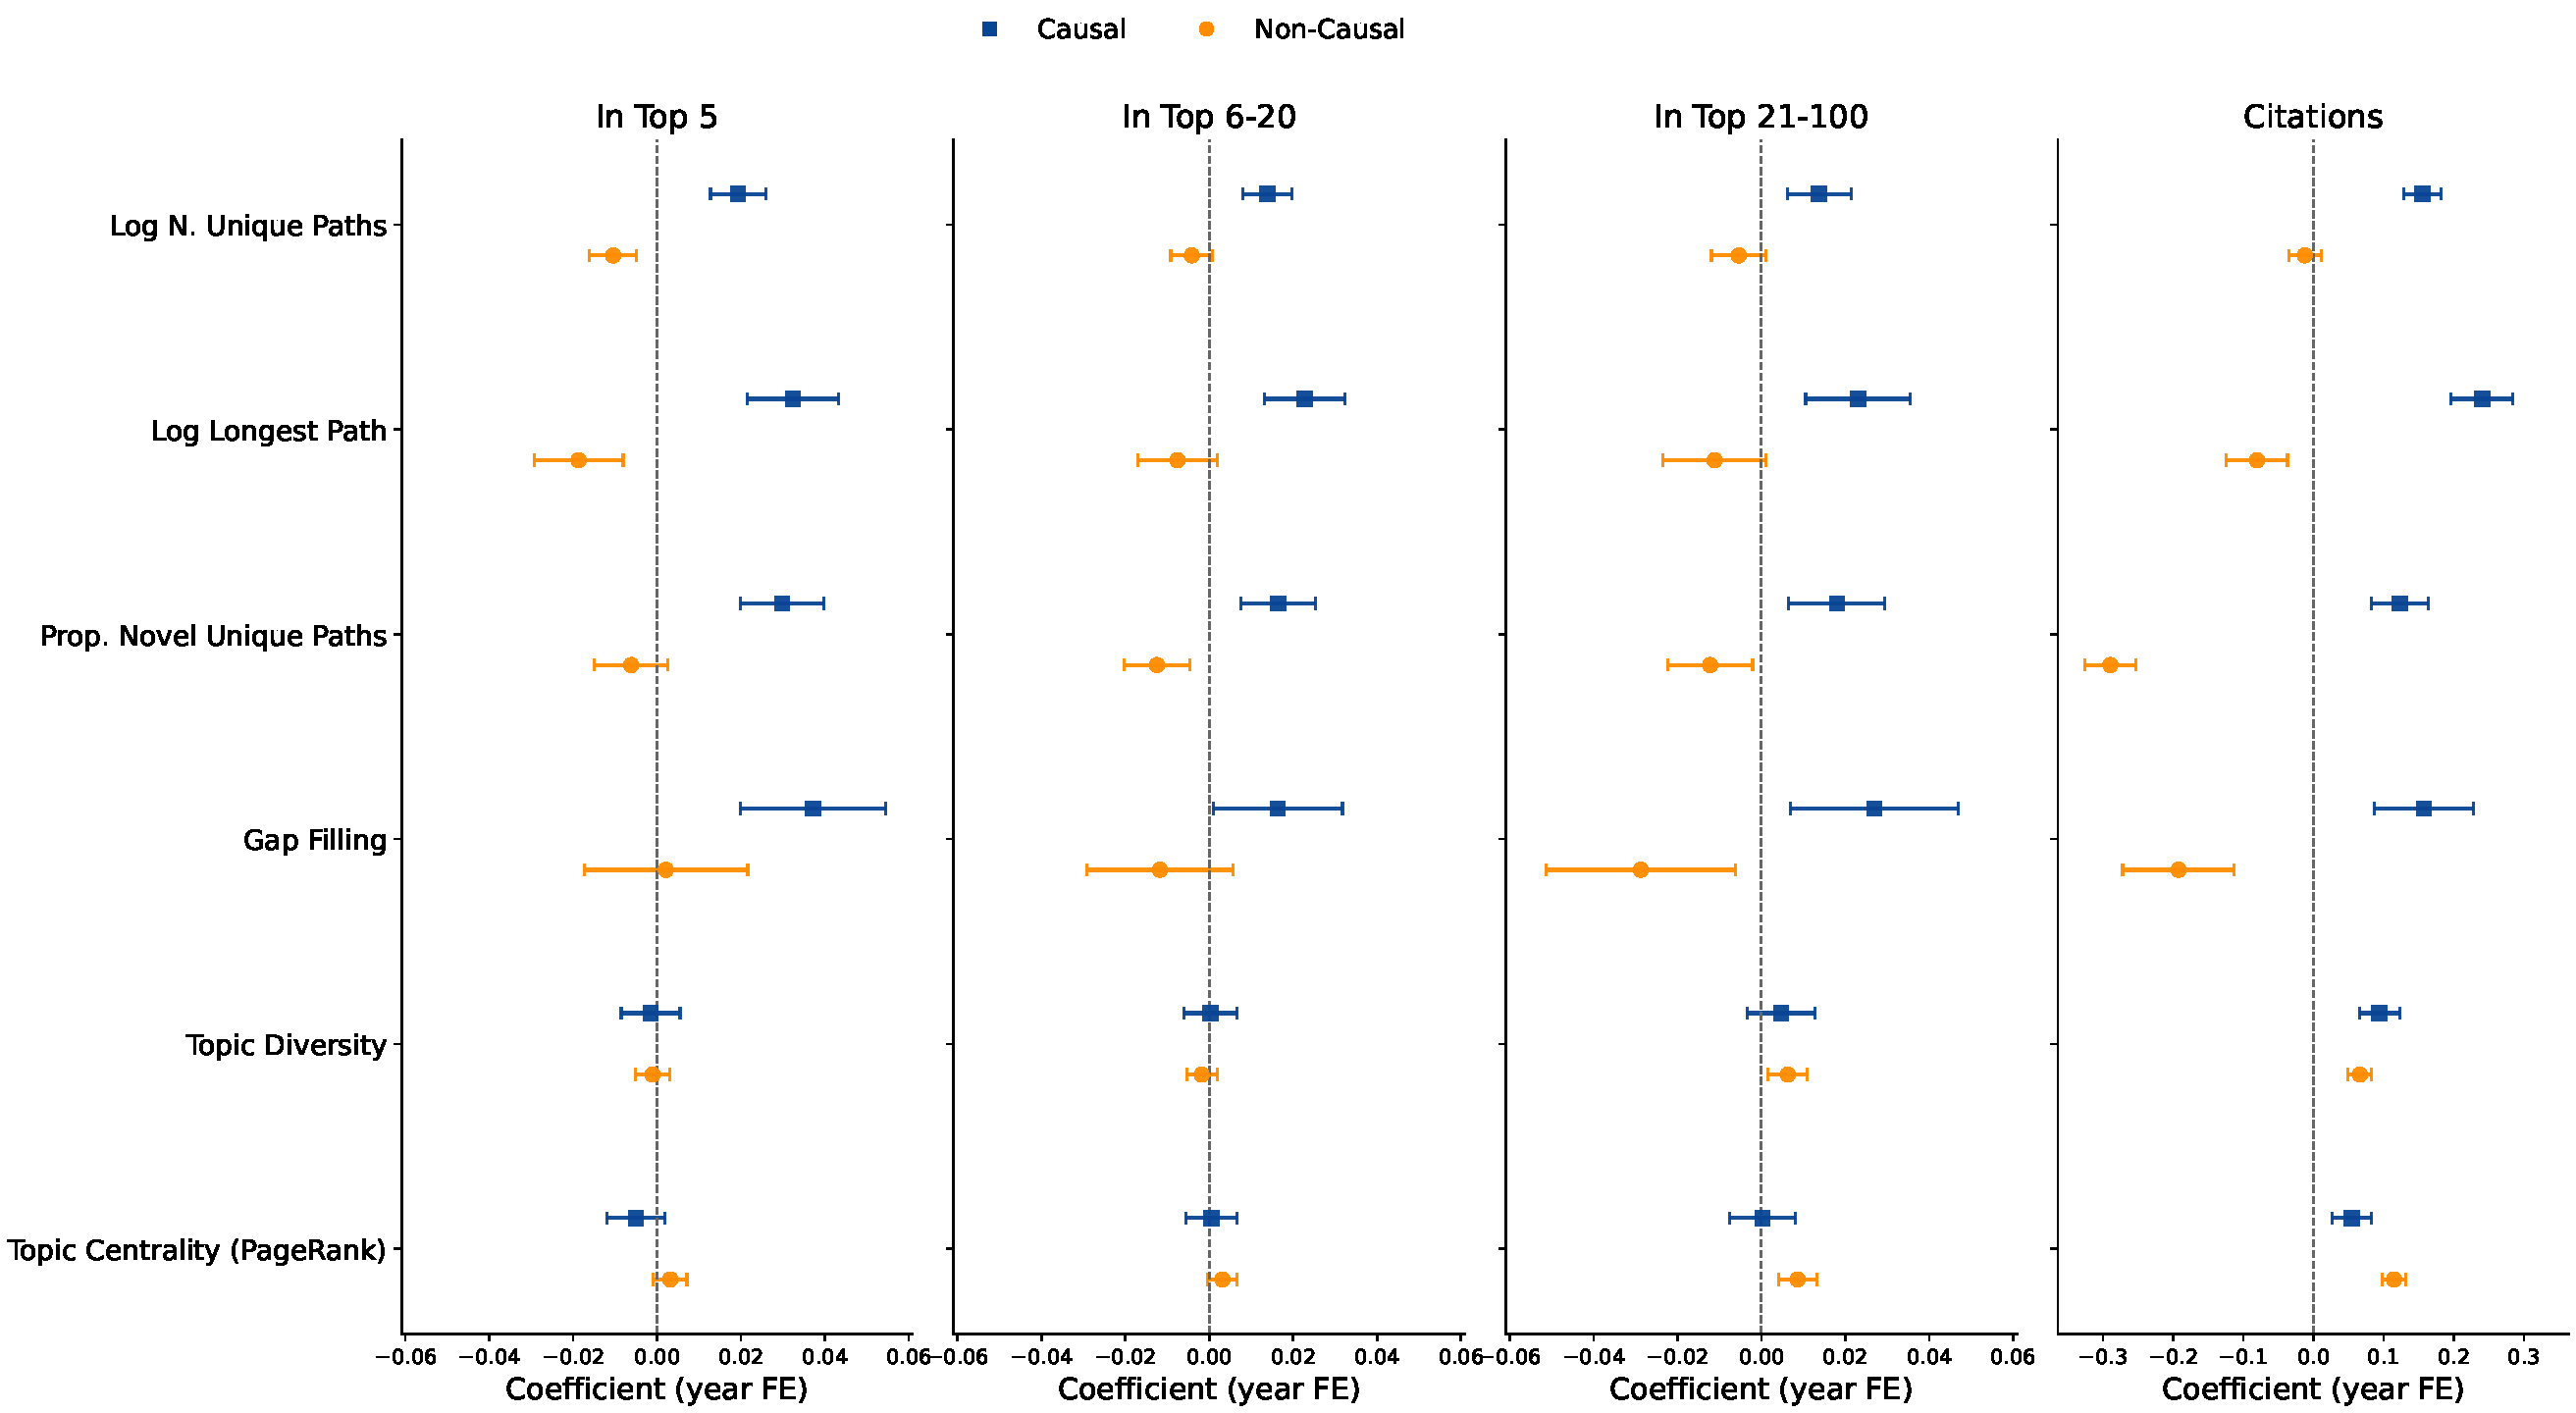
\includegraphics[width=0.88\linewidth,height=0.66\textheight,keepaspectratio]{publication_predictors_variants_appendix.pdf}};
  \end{tikzpicture}
  \figurecaptionbar{Variant measures for depth, path novelty, and topic diversity continue to favor causal over non-causal structure in top-tier placement and citations.}
\end{frame}

\begin{frame}[t]{Gap filling: top journals reward underexplored combinations unevenly}
  \hfill\BackButton{main-predictors}\par
  \vspace{0.08cm}
  \begin{columns}[T,onlytextwidth]
    \begin{column}{0.49\textwidth}
      \begin{tikzpicture}
        \node[
          fill=white,
          draw=LineSoft,
          rounded corners=10pt,
          inner sep=6pt
        ] {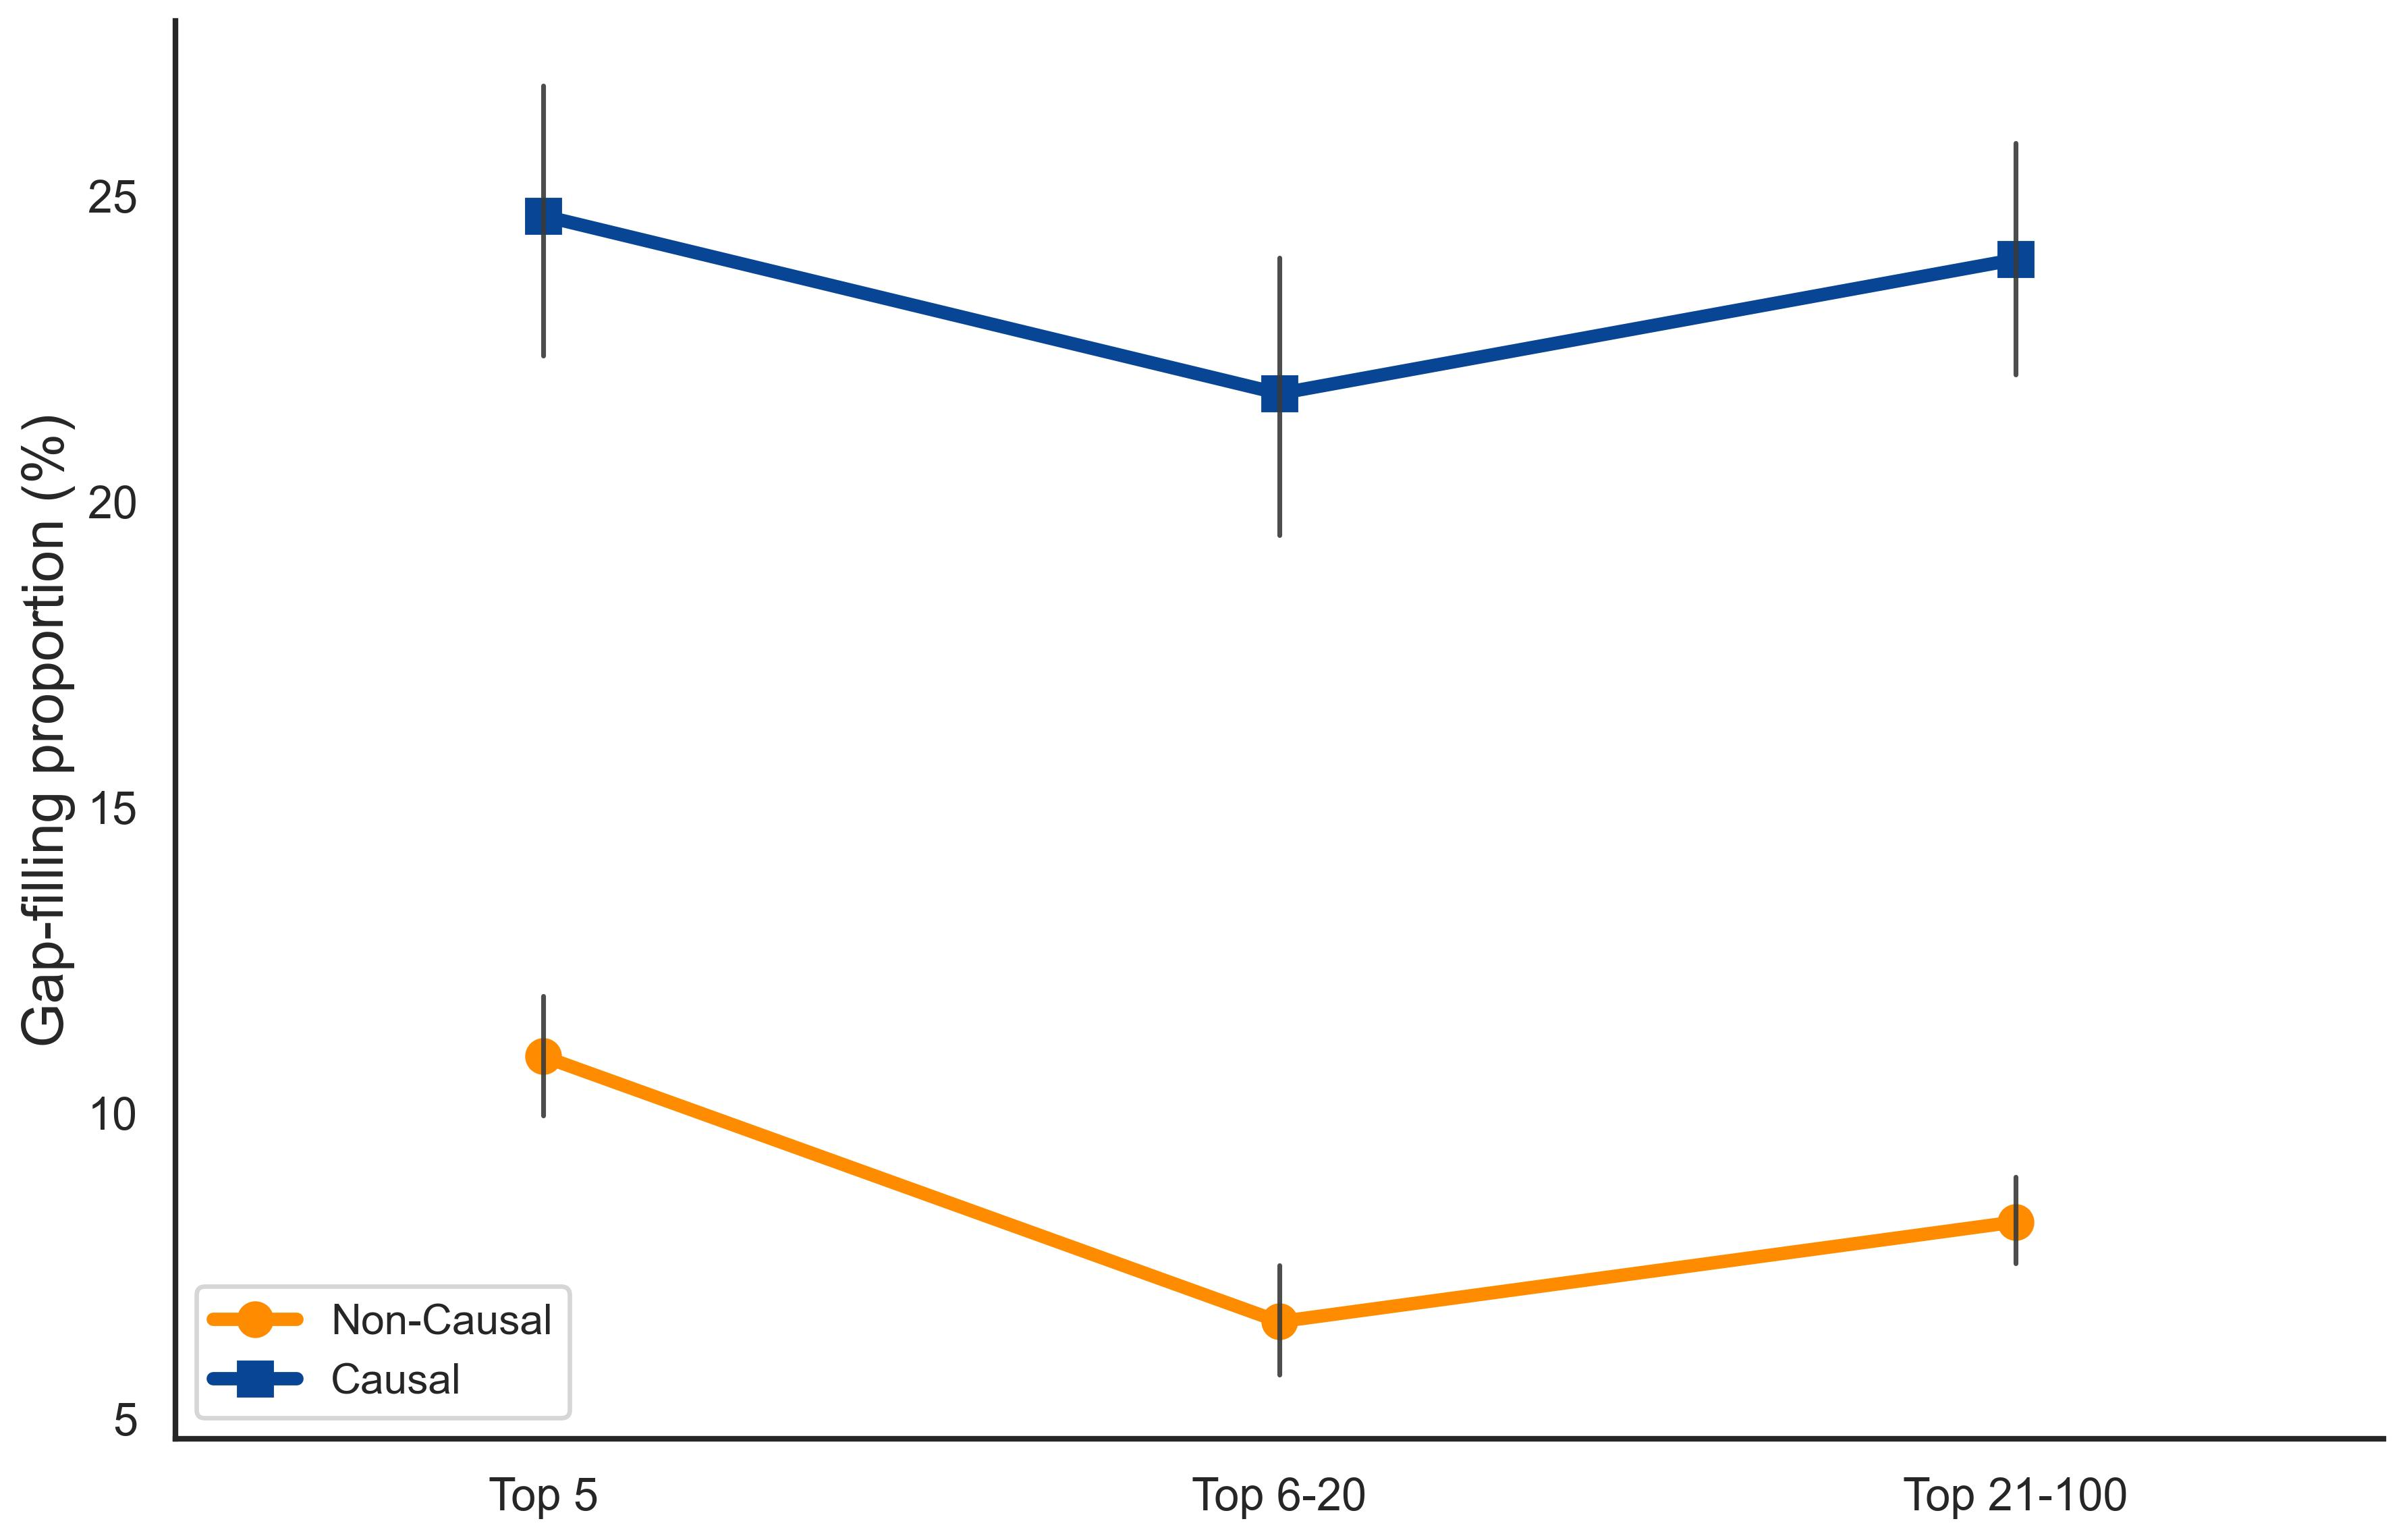
\includegraphics[width=0.94\linewidth]{gap_filling_journal_tiers_combined_non_causal.jpg}};
      \end{tikzpicture}
    \end{column}
    \begin{column}{0.49\textwidth}
      \begin{tikzpicture}
        \node[
          fill=white,
          draw=LineSoft,
          rounded corners=10pt,
          inner sep=6pt
        ] {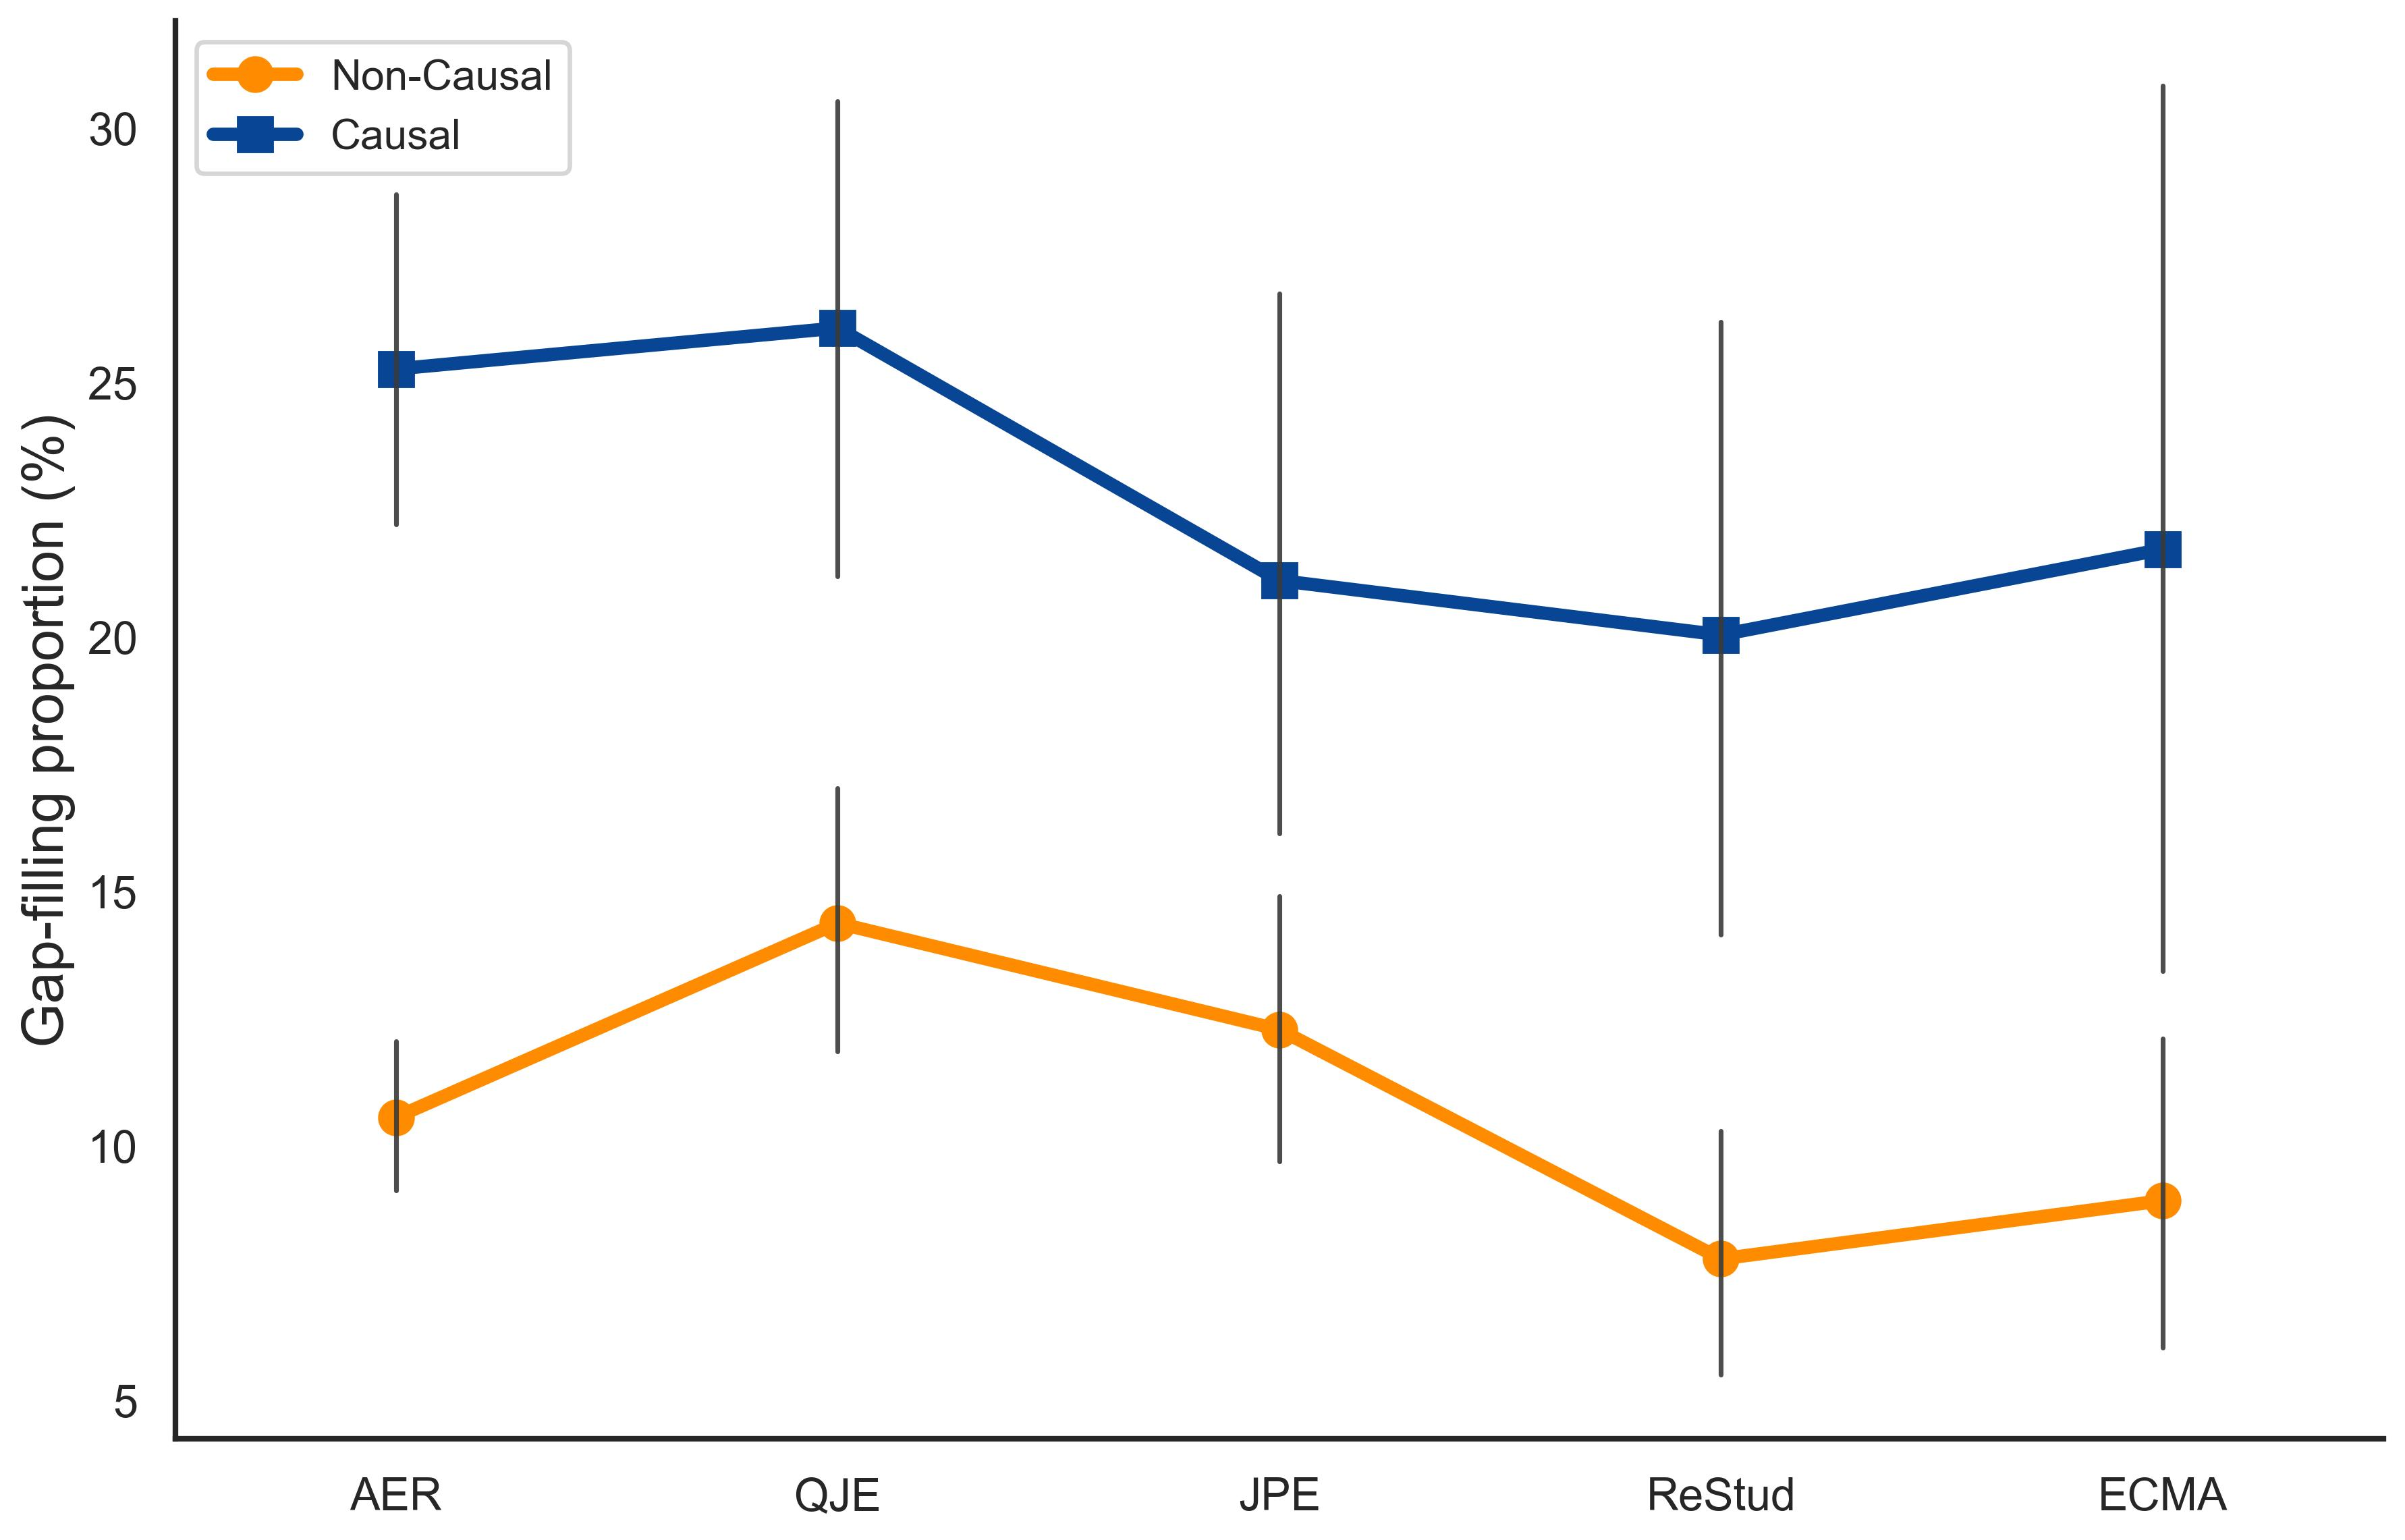
\includegraphics[width=0.94\linewidth]{gap_filling_top5_journals_combined_non_causal.jpg}};
      \end{tikzpicture}
    \end{column}
  \end{columns}
  \figurecaptionbar{Causal gap filling appears especially strong in journals like QJE and AER, but the citation payoff is less systematic than for causal depth or causal novelty.}
\end{frame}

\begin{frame}[t]{Validation summary in one slide}
  \hfill\BackButton{main-validation}\par
  \vspace{0.08cm}
  \begin{columns}[T,onlytextwidth]
    \begin{column}{0.32\textwidth}
      \Card{0.96\linewidth}{Brodeur benchmark}{
        Strong label recovery for several methods and fields; especially good performance for RDD, Macro, and Urban labels in matched papers.}
    \end{column}
    \begin{column}{0.32\textwidth}
      \Card{0.96\linewidth}{Plausibly exogenous benchmark}{
        High maximum semantic alignment for causes, effects, and especially sources of exogenous variation.}
    \end{column}
    \begin{column}{0.32\textwidth}
      \Card{0.96\linewidth}{Snippet audit}{
        Precision rises from roughly 0.78 to 0.94 as overlap thresholds tighten, with the expected recall trade-off.}
    \end{column}
  \end{columns}
  \figurecaptionbar{Together, the three checks cover label recovery, semantic alignment for exogenous variation, and precision--recall trade-offs inside the extraction pipeline.}
\end{frame}

\begin{frame}[t]{Data and replication notes}
  \begin{columns}[T,onlytextwidth]
    \begin{column}{0.48\textwidth}
      \Card{0.97\linewidth}{What is released}{
        Derived edge lists, paper-level measures, prompts, schemas, and analysis code via the \href{https://www.causal.claims/data-download}{project website}.}
    \end{column}
    \begin{column}{0.48\textwidth}
      \Card{0.97\linewidth}{What is not released}{
        Proprietary source PDFs are not redistributed, but the package supports regeneration once users re-download NBER and CEPR source documents.}
    \end{column}
  \end{columns}

  \vspace{0.35cm}
  \Card[PaperSand]{0.99\linewidth}{Why that matters}{
    The contribution is both a substantive finding and a reusable claim-level infrastructure for future meta-research.}
\end{frame}

\end{document}
